\documentclass[12pt,a4paper]{article}

% Khai bao cac package can thiet cho tieng Viet va can le
\usepackage[utf8]{inputenc}
\usepackage[T5]{fontenc}
\usepackage{geometry}
\usepackage{graphicx}
\usepackage{tikz}
\usepackage[hidelinks]{hyperref}
\usepackage[vietnamese]{babel}
\usepackage{indentfirst}
\usepackage{array}
\usepackage{float}
\usepackage{enumitem}
\usepackage{tabularx}
\usepackage{titletoc}
\usepackage{xltabular}


\usetikzlibrary{calc}
\setcounter{tocdepth}{3}
\renewcommand{\labelitemi}{$-$}
\renewcommand{\labelitemii}{$+$}


% Thiet lap kich thuoc le chuan cho trang bia
\geometry{
    top=25mm,
    bottom=25mm,
    left=35mm,
    right=20mm,
}

% ==================== CẤU HÌNH TỰ ĐỘNG ĐÁNH SỐ (TITLESEC) ====================
\usepackage{titlesec}

% Gan so thu tu hinh anh di kem voi so section
\counterwithin{figure}{section}

% Gan so thu tu bang bieu di kem voi so section
\counterwithin{table}{section}

% Cấu hình cho Section -> Biến thành "Chương X: Tên Chương" và CĂN GIỮA
\titleformat{\section}
  {\normalfont\Large\bfseries\centering}
  {Chương \thesection: }
  {0pt}
  {}

% Cấu hình cho Subsection -> Dạng "1.1. Tên mục" và CĂN TRÁI
\titleformat{\subsection}
  {\normalfont\large\bfseries}
  {\thesubsection.\ }
  {0pt}
  {}

% Cấu hình cho Subsubsection -> Dạng "1.1.1. Tên mục nhỏ" và CĂN TRÁI
\titleformat{\subsubsection}
  {\normalfont\normalsize\bfseries} 
  {  \thesubsubsection.\ }
  {0pt}
  {}

\titlecontents{section}
  [0em]
  {\bfseries\vspace{1ex}}
  {Chương \thecontentslabel: }
  {}
  {\titlerule*[0.3pc]{.}\contentspage}
% ==============================================================================

\begin{document}

% Bat dau moi truong trang bia
\begin{titlepage}
    \begin{tikzpicture}[remember picture, overlay]
        % Ve vien trong (cach le trai 3cm de dong gay, cac le khac 1.5cm)
        \draw[line width=1pt] 
            ($(current page.north west) + (3cm,-1.5cm)$) 
            rectangle 
            ($(current page.south east) + (-1.5cm,1.5cm)$);
            
        % Ve vien ngoai day hon (cach vien trong 0.1cm)
        \draw[line width=2.5pt] 
            ($(current page.north west) + (2.9cm,-1.4cm)$) 
            rectangle 
            ($(current page.south east) + (-1.4cm,1.4cm)$);
    \end{tikzpicture}
    \begin{center}
        % Header truong va khoa
        \Large \textbf{ĐẠI HỌC XÂY DỰNG HÀ NỘI}\\[0.1cm]
        \large \textbf{KHOA CÔNG NGHỆ THÔNG TIN}\\[0.1cm]
        {\large \rule{3.5cm}{0.5pt} \raisebox{-0.15ex}{o0o} \rule{3.5cm}{0.5pt}}\\[1cm]

        % Logo truong
        \vspace{1.5cm}
        
\includegraphics[width=4cm, keepaspectratio]{logo-huce.png}
        \vspace{1.5cm}
        
        % Ten cua bao cao/do an
        \Huge \textbf{CHYÊN ĐỀ TỔNG HỢP}\\[0.5cm]
        \large{NGÀNH: CÔNG NGHỆ THÔNG TIN}\\[0.5cm]
        \Large \textbf{Phát triển hệ thống blockchain riêng biệt cho một chuỗi doanh nghiệp}\\[2cm]
        
        % Can le phai cho thong tin nguoi thuc hien
        \textbf{Cấn Tất Dương}\\[1cm]
        
        % Day cac thanh phan tiep theo xuong day trang
        \vfill
        
        % Thong tin dia diem, thoi gian
        {\large Hà Nội, năm 2026}
    \end{center}
\end{titlepage}

% Bat dau moi truong trang bia
\begin{titlepage}
    \begin{tikzpicture}[remember picture, overlay]
        % Ve vien trong (cach le trai 3cm de dong gay, cac le khac 1.5cm)
        \draw[line width=1pt] 
            ($(current page.north west) + (3cm,-1.5cm)$) 
            rectangle 
            ($(current page.south east) + (-1.5cm,1.5cm)$);
            
        % Ve vien ngoai day hon (cach vien trong 0.1cm)
        \draw[line width=2.5pt] 
            ($(current page.north west) + (2.9cm,-1.4cm)$) 
            rectangle 
            ($(current page.south east) + (-1.4cm,1.4cm)$);
    \end{tikzpicture}
    \begin{center}
        % Header truong va khoa
        \Large \textbf{ĐẠI HỌC XÂY DỰNG HÀ NỘI}\\[0.1cm]
        \large \textbf{KHOA CÔNG NGHỆ THÔNG TIN}\\[0.1cm]
        {\large \rule{3.5cm}{0.5pt} \raisebox{-0.15ex}{o0o} \rule{3.5cm}{0.5pt}}\\[1cm]

        % Logo truong
        \vspace{1.5cm}
        
\includegraphics[width=4cm, keepaspectratio]{logo-huce.png}
        \vspace{1.5cm}
        
        % Ten cua bao cao/do an
        \Huge \textbf{CHYÊN ĐỀ TỔNG HỢP}\\[0.5cm]
        \large{NGÀNH: CÔNG NGHỆ THÔNG TIN}\\[0.5cm]
        \Large \textbf{Phát triển hệ thống blockchain riêng biệt cho một chuỗi doanh nghiệp}\\[2cm]
        
        % Can le phai cho thong tin nguoi thuc hien
        \textbf{Cấn Tất Dương}\\[1cm]

        GIÁO VIÊN HƯỚNG DẪN:\\
        \textbf{ThS. Nguyễn Việt Nhật}
        
        % Day cac thanh phan tiep theo xuong day trang
        \vfill
        
        % Thong tin dia diem, thoi gian
        {\large Hà Nội, năm 2026}
    \end{center}
\end{titlepage}

% ==================== LỜI CAM ĐOAN ====================
\section*{Lời cam đoan}
\addcontentsline{toc}{section}{Lời cam đoan}

Em xin cam đoan nội dung đồ án tốt nghiệp "Phát triển hệ thống blockchain riêng biệt cho một chuỗi doanh nghiệp" là do em tự nghiên cứu, tìm hiểu và thực hiện dưới sự hướng dẫn của Thầy Nguyễn Việt Nhật. 

Toàn bộ nội dung của đồ án không sao chép hay vay mượn trái phép từ các công trình khoa học khác. Các đoạn trích dẫn, số liệu và tài liệu tham khảo sử dụng trong báo cáo đều được trích dẫn nguồn gốc và ghi chú đầy đủ, rõ ràng trong danh mục tài liệu tham khảo.

Nếu phát hiện có bất kỳ sự gian lận hay sao chép nào, em xin chịu hoàn toàn trách nhiệm trước Hội đồng bảo vệ và nhà trường.

\vspace{1cm}
\begin{flushright}
    \begin{tabular}{c}
        \textit{Hà Nội, ngày ... tháng ... năm 2026} \\[0.5cm]
        \textbf{Sinh viên thực hiện} \\[2cm] % Bạn có thể chỉnh lại khoảng cách ký tại đây
        Cấn Tất Dương
    \end{tabular}
\end{flushright}

\newpage
% ==================== LỜI CẢM ƠN ====================
\section*{Lời cảm ơn}
\addcontentsline{toc}{section}{Lời cảm ơn}

Để hoàn thành được đồ án này, em xin gửi lời cảm ơn chân thành đến các thầy cô trong Khoa Công nghệ Thông tin - Trường Đại học Xây dựng Hà Nội đã tận tình giảng dạy và trang bị cho em những kiến thức nền tảng quý báu trong suốt bốn năm học vừa qua.

Đặc biệt, em xin bày tỏ lòng biết ơn sâu sắc đến Thầy Nguyễn Việt Nhật. Những bài giảng của thầy trong học phần An toàn bảo mật thông tin, cụ thể là việc đi sâu vào thuật toán mã hóa RSA, đã mở ra cho em những hiểu biết cốt lõi đầu tiên về hệ thống mật mã bất đối xứng (khóa công khai và khóa bí mật). Nền tảng tư duy vững chắc về bảo mật đó chính là kim chỉ nam giúp em có khả năng tự nghiên cứu, áp dụng chữ ký số đường cong Elliptic (Ed25519) \cite{bernstein} và trực tiếp lập trình cơ chế xác thực giao dịch an toàn cho lõi hệ thống ngày hôm nay.

Bên cạnh đó, em cũng xin gửi lời cảm ơn chân thành đến những người bạn và các anh chị đồng nghiệp đã luôn động viên, hỗ trợ và đóng góp các ý kiến quý báu trong suốt quá trình em phát triển mã nguồn cũng như hoàn thiện cuốn báo cáo này.

\vspace{1cm}
\begin{flushright}
    \begin{tabular}{c}
        \textbf{Sinh viên thực hiện} \\[2cm]
        Cấn Tất Dương
    \end{tabular}
\end{flushright}

\newpage
% ==================== LỜI NÓI ĐẦU ====================
\section*{Lời nói đầu}
\addcontentsline{toc}{section}{Lời nói đầu}

Trong bối cảnh nền kinh tế số đang phát triển mạnh mẽ, niềm tin và tính toàn vẹn của dữ liệu đã trở thành những tài sản vô hình mang tính sống còn đối với bất kỳ tổ chức nào. Công nghệ sổ cái phân tán (Blockchain) ra đời như một lời giải hoàn hảo cho bài toán đó, loại bỏ điểm lỗi duy nhất và minh bạch hóa mọi luồng thông tin. Tuy nhiên, sự phát triển của công nghệ này lại đang tạo ra một nghịch lý: các nền tảng Public thì chậm chạp và tốn kém, trong khi các giải pháp chuẩn công nghiệp (như Hyperledger Fabric) lại quá cồng kềnh, phức tạp và vượt quá khả năng chịu đựng về hạ tầng của phần lớn các doanh nghiệp vừa và nhỏ tại Việt Nam. 

Chính khoảng trống công nghệ đó đã thôi thúc em đặt ra một câu hỏi lớn: \textit{"Tại sao chúng ta không thể có một lõi blockchain đủ mạnh mẽ để bảo mật, nhưng lại đủ tinh gọn để khởi chạy trên một máy tính cá nhân?"} Đó là khởi nguồn cho đồ án \textbf{"Phát triển hệ thống blockchain riêng biệt cho một chuỗi doanh nghiệp (Khoai Chain)"}.

Đồ án này không đơn thuần là việc lắp ráp các công cụ có sẵn, mà là một hành trình đi sâu vào tầng cốt lõi của hệ thống phân tán. Việc tự tay thiết kế cấu trúc khối, viết logic cho mạng ngang hàng, và áp dụng các thuật toán mật mã để tự động hóa quá trình đồng thuận mang lại những thách thức rất lớn, nhưng cũng là những trải nghiệm học thuật giá trị nhất. Từ triết lý "tối giản hóa", được thiết kế nhằm mang lại một môi trường thử nghiệm độc lập, dễ dàng đóng gói và triển khai, giúp thu hẹp khoảng cách giữa lý thuyết mật mã học phức tạp và khả năng ứng dụng thực chiến trong doanh nghiệp.

Dù hệ thống đã hình thành được bộ khung kiến trúc và đáp ứng được các luồng giao dịch cơ bản, nhưng với giới hạn về mặt thời gian cũng như kinh nghiệm vận hành thực tiễn, mã nguồn của chắc chắn vẫn còn những góc khuất chưa được tối ưu triệt để (như giới hạn tài nguyên tính toán hay cơ chế tự động tái cấu trúc chuỗi). Em rất mong nhận được những nhận xét, đánh giá khắt khe và các lời góp ý quý báu từ Hội đồng bảo vệ để có thể tiếp tục hoàn thiện, nâng cấp hệ thống vững chắc hơn trong tương lai.

\newpage

% Mục lục tự động tạo dựa trên các section, subsection phía dưới
\addcontentsline{toc}{section}{Mục lục}
\tableofcontents
% Danh muc hinh ve
\newpage
\addcontentsline{toc}{section}{Danh mục hình vẽ}
\listoffigures

% Danh muc bang bieu
\newpage
\addcontentsline{toc}{section}{Danh mục bảng biểu}
\listoftables
\newpage

\newpage
\section*{Danh mục từ viết tắt, thuật ngữ}
\addcontentsline{toc}{section}{Danh mục từ viết tắt, thuật ngữ}

% Bang danh muc tu viet tat da duoc cap nhat day du và sap xep theo thu tu bang chu cai
\renewcommand{\arraystretch}{1.5}
\begin{xltabular}{\textwidth}{|c|l|X|}
    \hline
    \textbf{STT} & \textbf{Từ viết tắt, thuật ngữ} & \textbf{Giải nghĩa} \\ \hline
    1 & API & Giao diện lập trình ứng dụng (Application Programming Interface) \\ \hline
    2 & BFT & Dung sai lỗi Byzantine (Byzantine Fault Tolerance) \\ \hline
    3 & CA & Tổ chức cấp chứng chỉ (Certificate Authority) \\ \hline
    4 & CFT & Dung sai lỗi hỏng hóc (Crash Fault Tolerance) \\ \hline
    5 & CLI & Giao diện dòng lệnh (Command-Line Interface) \\ \hline
    6 & CPU & Bộ vi xử lý trung tâm \\ \hline
    7 & DHT & Bảng băm phân tán (Distributed Hash Table) \\ \hline
    8 & DLT & Công nghệ sổ cái phân tán (Distributed Ledger Technology) \\ \hline
    9 & DX & Trải nghiệm dành cho nhà phát triển (Developer Experience) \\ \hline
    10 & ECDSA & Thuật toán chữ ký số dựa trên đường cong Elliptic (Elliptic Curve Digital Signature Algorithm) \\ \hline
    11 & EVM & Máy ảo Ethereum (Ethereum Virtual Machine) \\ \hline
    12 & I/O & Input/Output \\ \hline
    13 & IBFT & Istanbul Byzantine Fault Tolerance \\ \hline
    14 & ID & Mã định danh (Identifier) \\ \hline
    15 & JSON & JavaScript Object Notation \\ \hline
    16 & P2P & Mạng ngang hàng (Peer-to-Peer) \\ \hline
    17 & PBFT & Practical Byzantine Fault Tolerance \\ \hline
    18 & PoA & Bằng chứng ủy quyền (Proof of Authority) \\ \hline
    19 & PoS & Bằng chứng cổ phần (Proof of Stake) \\ \hline
    20 & PoW & Bằng chứng công việc (Proof of Work) \\ \hline
    21 & RAM & Bộ nhớ trong \\ \hline
    22 & RPC & Remote Procedure Call \\ \hline
    23 & RSA & Thuật toán mã hóa bất đối xứng Rivest-Shamir-Adleman \\ \hline
    24 & SDK & Bộ công cụ phát triển phần mềm (Software Development Kit) \\ \hline
    25 & SHA-256 & Thuật toán băm an toàn 256-bit (Secure Hash Algorithm 256-bit) \\ \hline
    26 & SME & Doanh nghiệp vừa và nhỏ (Small and Medium-sized Enterprises) \\ \hline
    27 & SPOF & Điểm lỗi duy nhất (Single Point of Failure) \\ \hline
    28 & TCP/IP & Giao thức điều khiển truyền vận/Giao thức Internet \\ \hline
    29 & TPS & Tốc độ xử lý giao dịch (Transactions Per Second) \\ \hline
    30 & VPS & Máy chủ ảo (Virtual Private Server) \\ \hline
\end{xltabular}

\newpage


% ==================== THÂN BÀI: TỰ ĐỘNG ĐÁNH SỐ HOÀN TOÀN ====================

\section{Giới thiệu đề tài} % Máy tự hiện: Chương 1: Giới thiệu đề tài (Căn giữa)

\begin{figure}[H]
    \centering
    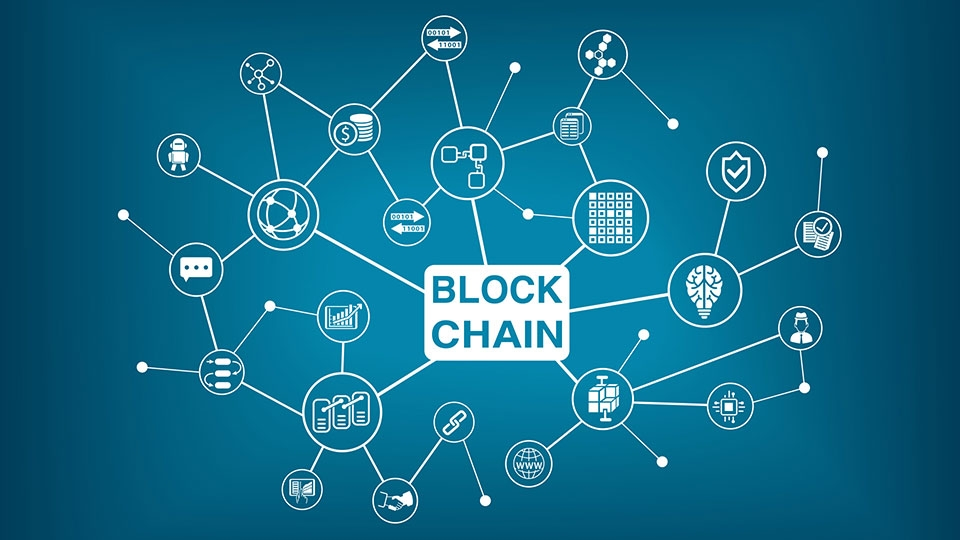
\includegraphics[width=1\textwidth]{Image/blockchain.png}
    \caption{Công nghệ blockchain}
    \label{fig:blockchain}
\end{figure}

\subsection{Lý do chọn đề tài}

\subsubsection{Sự phức tạp và cồng kềnh của các nền tảng blockchain hiện tại}
% Lồng ghép bài toán chuỗi cung ứng thuốc vào để làm dẫn chứng
Từ thực tiễn triển khai các bài toán nghiệp vụ phức tạp, điển hình như hệ thống quản lý chuỗi cung ứng thuốc trên nền tảng như Hyperledger Fabric, công nghệ này bộc lộ rõ những rào cản lớn về mặt kỹ thuật và vận hành. Cụ thể, kiến trúc của Fabric đòi hỏi tài nguyên phần cứng đồ sộ để duy trì các thành phần độc lập (như Orderer, Peer, CA) và yêu cầu thiết lập hệ thống chứng chỉ số phức tạp \cite{fabric}. Quá trình cấu hình, gỡ lỗi và triển khai mạng lưới tốn rất nhiều thời gian, trở thành một nút thắt lớn (bottleneck) cho các nhà phát triển. Sự cồng kềnh này hoàn toàn không phù hợp với các mô hình thử nghiệm nhanh, các dự án giáo dục, hoặc các doanh nghiệp có hạ tầng hạn chế, từ đó đặt ra yêu cầu cấp thiết về một nền tảng blockchain tinh gọn hơn nhưng vẫn đảm bảo tính bất biến của dữ liệu.

\subsubsection{Nhu cầu về một hệ thống blockchain thử nghiệm}
% Tập trung vào môi trường giáo dục và phát triển, tách biệt SDK và Core
Từ góc độ nghiên cứu và giáo dục, việc tiếp cận kiến trúc blockchain doanh nghiệp hiện nay gặp rất nhiều trở ngại do yêu cầu khắt khe về phần cứng. Người học và nhà phát triển thiếu đi một môi trường thử nghiệm tinh gọn, nơi họ có thể nhanh chóng khởi tạo một mạng lưới blockchain độc lập ngay trên máy tính cá nhân. Nhu cầu thực tế đòi hỏi một hệ thống được đóng gói nhẹ nhàng, đi kèm với các bộ công cụ phát triển (SDK) được tách biệt rõ ràng. Điều này giúp sinh viên và lập trình viên tập trung hoàn toàn vào việc xây dựng logic nghiệp vụ thông qua Hợp đồng thông minh, thay vì tốn thời gian xử lý các cấu hình mạng ngang hàng hay cơ chế đồng thuận ở tầng lõi.

\subsubsection{Nhu cầu thực tiễn của doanh nghiệp vừa và nhỏ}
% Giải quyết bài toán cân bằng giữa tính minh bạch và chi phí vận hành cho SME
Các doanh nghiệp vừa và nhỏ hoặc các chuỗi cung ứng quy mô nội bộ luôn có nhu cầu ứng dụng blockchain để giải quyết bài toán minh bạch hóa dữ liệu, chống giả mạo thông tin và truy xuất nguồn gốc. Mặc dù vậy, bài toán chi phí hạ tầng của các giải pháp chuẩn công nghiệp thường vượt quá khả năng đáp ứng của họ. Nhóm doanh nghiệp này cần một giải pháp blockchain được thiết kế tối giản nhưng vẫn giữ nguyên các đặc tính cốt lõi của sổ cái phân tán. Việc phát triển một hệ thống blockchain riêng biệt, có khả năng "cắm và chạy", tiêu tốn ít tài nguyên và dễ dàng tích hợp vào cơ sở hạ tầng máy chủ hiện có, sẽ giải quyết triệt để rào cản chi phí đồng thời bảo vệ an toàn cho các dữ liệu nhạy cảm của doanh nghiệp.

\subsection{Mục tiêu nghiên cứu}
Đề tài hướng tới việc giải quyết những rào cản kỹ thuật của các nền tảng sổ cái phân tán truyền thống bằng cách xây dựng một hệ thống tinh gọn. Mục tiêu tổng thể được chia thành hai khía cạnh chính nhằm phục vụ cả môi trường nghiên cứu học thuật lẫn ứng dụng thực tiễn.

\subsubsection{Tối ưu hóa quá trình triển khai và khởi chạy node}
Hệ thống được thiết kế để giảm thiểu tối đa các bước thiết lập môi trường phức tạp. Bằng cách phát triển các công cụ giao diện dòng lệnh và đóng gói toàn bộ quy trình khởi chạy dưới dạng các container, mục tiêu là cho phép người dùng có thể kích hoạt một node mạng lưới độc lập chỉ bằng vài thao tác cơ bản. Quá trình triển khai tự động này loại bỏ sự phụ thuộc vào các dịch vụ hạ tầng trung gian, giúp việc kết nối vào mạng ngang hàng, thử nghiệm cục bộ và gỡ lỗi diễn ra nhanh chóng. Điều này đặc biệt hữu ích trong việc tiết kiệm tài nguyên tính toán, cho phép chạy mượt mà ngay trên các thiết bị máy tính cá nhân tiêu chuẩn.

\subsubsection{Xây dựng lõi blockchain chuyên biệt hóa cho chuỗi doanh nghiệp}
Mục tiêu trọng tâm là phát triển một lõi được tinh chỉnh trực tiếp cho các luồng nghiệp vụ nội bộ. Kiến trúc lõi sẽ tự chủ hoàn toàn các thành phần như quản lý mempool, đồng bộ block, giao thức P2P và định tuyến giao dịch. Bằng cách cung cấp một môi trường thực thi được cô lập và tách biệt qua bộ SDK, các nhà phát triển có thể trực tiếp ánh xạ các quy tắc kinh doanh thành Hợp đồng thông minh mà không làm ảnh hưởng đến tính ổn định của toàn mạng. Khác với kiến trúc phục vụ đám đông, hệ thống lõi này chuyên biệt hóa cho một nhóm các định chế hoặc đối tác kinh doanh đã được xác thực, đảm bảo giao dịch được lưu vết minh bạch, nhất quán nhưng vẫn nằm trong phạm vi giới hạn an toàn của chuỗi.
\newpage
\subsection{Đối tượng và phạm vi nghiên cứu}
% Xác định rõ đối tượng kỹ thuật và ranh giới giới hạn của đề tài
\textbf{Đối tượng nghiên cứu của đề tài là công nghệ sổ cái phân tán, mạng ngang hàng và cơ chế thực thi hợp đồng thông minh.}

Phạm vi nghiên cứu tập trung vào việc thiết kế và xây dựng lõi hệ thống từ đầu, giới hạn trong môi trường mạng nội bộ phục vụ chuỗi doanh nghiệp vừa và nhỏ hoặc mục đích giáo dục. Đề tài không tập trung giải quyết các bài toán của public blockchain như phát hành tiền mã hóa, khai thác, hay khả năng mở rộng hàng triệu người dùng.

\newpage

\section{Cơ sở lý thuyết và Công nghệ nền tảng}

\subsection{Tổng quan về công nghệ Blockchain}

\subsubsection{Khái niệm và nguyên lý hoạt động cơ bản}
Blockchain là một công nghệ sổ cái phân tán cho phép ghi lại các giao dịch một cách an toàn, minh bạch và không thể đảo ngược trên một mạng lưới máy tính ngang hàng. Thay vì lưu trữ dữ liệu tại một máy chủ trung tâm, dữ liệu của blockchain được nhân bản và đồng bộ hóa tại tất cả các nút tham gia mạng lưới \cite{antonopoulos}.

Cấu trúc lưu trữ dữ liệu của Blockchain bao gồm chuỗi các khối liên kết tuyến tính với nhau theo thời gian. Mỗi khối chứa hai thành phần chính:
\begin{itemize}
    \item \textbf{Phần đầu khối:} Chứa siêu dữ liệu quản lý khối, bao gồm:
    \begin{itemize}
        \item \textbf{Phiên bản:} Phiên bản của giao thức blockchain.
        \item \textbf{Mã băm khối trước:} Mã băm của toàn bộ header khối trước đó. Đây là sợi xích toán học liên kết các khối. Nếu dữ liệu khối trước bị sửa đổi, mã băm này thay đổi và làm gãy toàn bộ chuỗi phía sau.
        \item \textbf{Mã băm gốc Merkle:} Mã băm gốc của cây Merkle, đại diện cho toàn bộ giao dịch trong khối \cite{antonopoulos}.
        \item \textbf{Mốc thời gian:} Thời gian khối được tạo ra.
        \item \textbf{Nonce và bits:} Các tham số phục vụ cho cơ chế đồng thuận (ví dụ trong bằng chứng công việc).
    \end{itemize}
    \item \textbf{Thân khối:} Chứa danh sách chi tiết các giao dịch thực tế đã được xác thực và đóng gói vào khối.
\end{itemize}

\subsubsection{Các đặc trưng cốt lõi của Blockchain}
\begin{itemize}
    \item \textbf{Tính phân tán:} Hệ thống loại bỏ thực thể trung tâm quản lý. Quyền lực ghi và xác thực sổ cái được chia đều cho các nút trong mạng theo luật đồng thuận, giúp loại bỏ điểm lỗi duy nhất (SPOF) \cite{antonopoulos}.
    \item \textbf{Tính minh bạch:} Mọi tài khoản tham gia mạng lưới đều có quyền truy cập, tra cứu và kiểm toán toàn bộ lịch sử giao dịch từ khối khởi thủy đến khối hiện tại.
    \item \textbf{Tính bất biến:} Dữ liệu một khi đã được đồng thuận ghi vào chuỗi thì không thể sửa đổi hoặc xóa bỏ. Muốn thay đổi một khối, kẻ tấn công phải thay đổi tất cả các khối sau nó và chiếm trên 51\% sức mạnh toán học hoặc quyền kiểm soát mạng lưới, điều này bất khả thi về mặt chi phí trong các mạng lớn.
    \item \textbf{Khả năng truy xuất:} Nhờ cơ chế liên kết mã băm và mốc thời gian cố định, mọi thực thể dữ liệu hoặc tài sản số hóa lưu trữ trên blockchain đều có thể được truy vết nguồn gốc dịch chuyển một cách chính xác qua từng địa chỉ ví.
\end{itemize}

\subsubsection{Phân loại mạng lưới Blockchain}
\begin{itemize}
    \item \textbf{Blockchain công khai:} Bất kỳ ai cũng có thể tham gia đọc, ghi dữ liệu và tham gia vào quá trình đồng thuận (ví dụ: Bitcoin, Ethereum). Mạng này có tính phi tập trung tối đa nhưng tốc độ xử lý giao dịch thấp và chi phí vận hành lớn.
    \item \textbf{Blockchain riêng tư:} Quyền đọc, ghi và đồng thuận hoàn toàn thuộc về một tổ chức duy nhất quản lý. Tốc độ xử lý rất nhanh, bảo mật nội bộ cao, nhưng mang tính tập trung cao.
    \item \textbf{Blockchain liên minh:} Quyền kiểm soát mạng lưới được chia sẻ cho một nhóm các tổ chức hoặc doanh nghiệp có lợi ích chung (ví dụ: liên minh ngân hàng, chuỗi cung ứng).
\end{itemize}
\textbf{Mối liên hệ với đề tài:} Đối với các bài toán chuỗi doanh nghiệp, blockchain liên minh hoặc blockchain riêng tư như Hyperledger Fabric là mô hình tối ưu nhất. Nó vừa giữ được tính minh bạch và bất biến của blockchain giữa các bên đối tác, vừa giải quyết được bài toán bảo mật dữ liệu kinh doanh, kiểm soát quyền truy cập nghiêm ngặt và đạt hiệu năng xử lý cao đáp ứng quy mô công nghiệp.

\subsection{Cơ sở mật mã học trong Blockchain}

\subsubsection{Hàm băm mật mã}
Hàm băm mật mã là một thuật toán toán học chuyển đổi một đầu vào dữ liệu có kích thước bất kỳ thành một chuỗi ký tự đầu ra có độ dài cố định. Trong các hệ thống blockchain, thuật toán SHA-256 (Secure Hash Algorithm 256-bit, dùng trong Bitcoin) hoặc Keccak256 (dùng trong Ethereum) được áp dụng phổ biến. Một hàm băm mật mã học tiêu chuẩn bắt buộc phải đảm bảo 3 đặc tính cốt lõi sau:
\begin{itemize}
    \item \textbf{Tính tất định:} Với cùng một thông điệp đầu vào $M$, hàm băm luôn luôn trả về một kết quả đầu ra $H(M)$ duy nhất, không thay đổi qua các lần tính toán.
    \item \textbf{Tính một chiều:} Khi biết trước một giá trị băm $Y$, về mặt toán học cực kỳ khó khăn (bất khả thi trong thời gian thực) để tìm lại thông điệp gốc $X$ sao cho $H(X) = Y$. Cách duy nhất là thử sai ngẫu nhiên.
    \item \textbf{Tính kháng va chạm:} Cực kỳ khó để tìm thấy hai thông điệp khác nhau hoàn toàn $X_1$ và $X_2$ mà khi băm lại cho ra cùng một kết quả ($H(X_1) = H(X_2)$). Ngoài ra, hàm băm có hiệu ứng tuyết lở: chỉ cần thay đổi 1 bit ở đầu vào, toàn bộ chuỗi đầu ra sẽ thay đổi hoàn toàn \cite{stallings}.
\end{itemize}

\subsubsection{Chữ ký số và mã hóa bất đối xứng}
Mã hóa bất đối xứng sử dụng một cặp khóa toán học liên kết chặt chẽ với nhau: khóa riêng dùng để tạo chữ ký số và khóa công khai dùng để xác thực chữ ký hoặc định danh địa chỉ ví.

Trong blockchain, thuật toán ECDSA - thuật toán chữ ký số dựa trên đường cong elliptic - được áp dụng để tối ưu hóa kích thước khóa và tốc độ tính toán so với RSA truyền thống.
\begin{itemize}
    \item \textbf{Quy trình ký:} Khi người dùng muốn thực hiện giao dịch, họ dùng khóa riêng của mình kết hợp với mã băm của nội dung giao dịch thông qua thuật toán ECDSA để tạo ra một chuỗi chữ ký số ($Sig$).
    \item \textbf{Quy trình xác thực:} Các nút trong mạng nhận được giao dịch sẽ dùng khóa công khai của người gửi để giải mã và kiểm tra tính hợp lệ của $Sig$. Quy trình này chứng minh người gửi sở hữu tài khoản và đồng ý chuyển tiền mà không cần tiết lộ khóa riêng cho mạng lưới, ngăn chặn hoàn toàn việc giả mạo giao dịch.
\end{itemize}
\newpage
\subsection{Mạng ngang hàng}

\subsubsection{Kiến trúc máy khách - máy chủ so với mạng ngang hàng}
\begin{figure}[H]
    \centering
    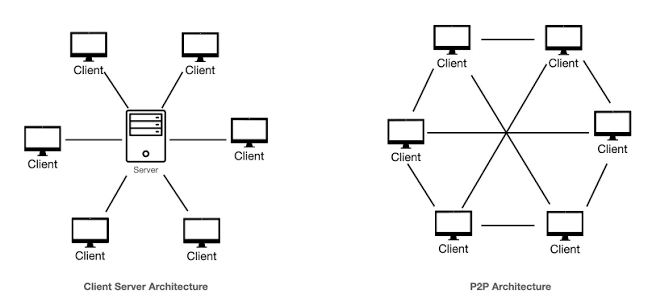
\includegraphics[width=1\textwidth]{Image/p2p.png}
    \caption{Máy khách/máy chủ so với mạng ngang hàng}
    \label{fig:p2p}
\end{figure}
\begin{itemize}
    \item \textbf{Kiến trúc máy khách - máy chủ:} Dữ liệu tập trung hoàn toàn tại hệ thống máy chủ. Các máy trạm muốn tương tác đều phải gửi yêu cầu về máy chủ. Kiến trúc này chịu nhược điểm điểm lỗi duy nhất (SPOF): nếu máy chủ bị sập, bị tấn công DDoS, hoặc bị hack dữ liệu, toàn bộ hệ thống sẽ tê liệt và dữ liệu có nguy cơ bị thao túng hoàn toàn.
    \item \textbf{Kiến trúc mạng ngang hàng:} Mạng lưới bao gồm các nút có vai trò và quyền hạn ngang hàng nhau. Mỗi nút vừa hoạt động như một máy khách (yêu cầu dữ liệu) vừa như một máy chủ (cung cấp, lưu trữ, xác thực dữ liệu). Khi một số nút bị ngắt kết nối hoặc bị tấn công, hệ thống vẫn vận hành bình thường nhờ các bản sao tại các nút còn lại, loại bỏ hoàn toàn bài toán điểm lỗi duy nhất.
\end{itemize}

\subsubsection{Giao thức truyền bá thông điệp}
Giao thức truyền bá thông điệp là cơ chế giao tiếp chính giúp các nút trong mạng lưới ngang hàng phi tập trung có thể phát tán thông tin (như giao dịch mới hoặc khối mới tạo) ra toàn mạng một cách nhanh chóng và tiết kiệm băng thông.
\begin{itemize}
    \item \textbf{Nguyên lý hoạt động:} Khi một nút nhận được một thông điệp mới, nó sẽ chọn ngẫu nhiên một số lượng nút K hàng xóm để chuyển tiếp thông điệp đó. Các nút nhận tiếp theo lại lặp lại quy trình chọn ngẫu nhiên này.
    \item \textbf{Hiệu quả:} Thông tin được lan truyền theo cấp số nhân. Chỉ trong một thời gian cực ngắn với độ phức tạp thời gian là $O(\log N)$ \cite{demers} (với $N$ là tổng số nút), toàn bộ mạng lưới rộng lớn sẽ đạt được trạng thái đồng bộ thông tin mà không cần một máy chủ điều phối trung tâm điều hướng luồng tin.
\end{itemize}

\subsection{Cơ chế đồng thuận}

\subsubsection{Bài toán tướng Byzantine}
Được đặt ra bởi Lamport, Shostak và Pease vào năm 1982 \cite{lamport}, bài toán mô tả một nhóm các vị tướng Byzantine vây hãm một thành phố địch. Họ liên lạc với nhau chỉ bằng tin nhắn messenger. Các tướng phải đồng thuận về một kế hoạch duy nhất: cùng tấn công hoặc cùng rút lui. Nếu có một vài tướng phản bội (hoặc tin nhắn bị thất lạc), họ sẽ cố tình gửi các thông điệp mâu thuẫn (gửi "tấn công" cho tướng này nhưng gửi "rút lui" cho tướng khác) nhằm làm chia rẽ và thất bại quân đội.

\textbf{Ý nghĩa trong blockchain:} Đây là mô hình hóa thách thức đạt được sự đồng thuận dữ liệu trong một hệ thống phân tán, nơi các nút tham gia mạng có thể bị lỗi kỹ thuật, mất kết nối, hoặc tệ hơn là chủ động gian lận, gửi dữ liệu sai lệch để trục lợi.

\subsubsection{Các thuật toán đồng thuận truyền thống}
\begin{itemize}
    \item \textbf{Bằng chứng công việc (PoW):} Các nút phải cạnh tranh giải một bài toán toán học cực khó bằng sức mạnh phần cứng máy tính (tìm giá trị nonce thích hợp). Người đầu tiên giải được sẽ giành quyền đóng gói khối và nhận phần thưởng \cite{antonopoulos}. Bằng chứng công việc bảo mật rất cao nhưng tiêu tốn tài nguyên điện năng khổng lồ và tốc độ xử lý giao dịch rất chậm (Bitcoin chỉ khoảng 7 TPS).
    \item \textbf{Bằng chứng cổ phần (PoS):} Thay thế việc khai thác bằng phần cứng bằng việc đặt cọc tiền điện tử. Hệ thống dựa vào tỷ lệ cổ phần đặt cọc để chọn ngẫu nhiên nút có quyền tạo khối mới. Bằng chứng cổ phần tiết kiệm năng lượng hơn bằng chứng công việc, tốc độ nhanh hơn, nhưng có nguy cơ dẫn đến việc tích lũy tài sản (người giàu càng giàu và nắm quyền kiểm soát mạng).
    \item \textbf{Bằng chứng ủy quyền (PoA):} Thay vì sử dụng năng lực tính toán hay lượng tiền đặt cọc, cơ chế này dựa trên danh tính và uy tín của các nút xác thực. Chỉ một nhóm các nút đã được kiểm duyệt, định danh và cấp phép từ trước mới có quyền đóng gói khối. Bằng chứng ủy quyền mang lại tốc độ xử lý giao dịch cực kỳ cao, gần như không tiêu tốn tài nguyên phần cứng và rất phù hợp cho các mạng blockchain riêng tư hoặc blockchain liên minh; tuy nhiên phải đánh đổi bằng việc mang tính tập trung cao hơn so với bằng chứng công việc hay bằng chứng cổ phần.
\end{itemize}

\newpage
\subsubsection{Đồng thuận trong blockchain riêng tư}
Hệ thống chuỗi doanh nghiệp yêu cầu tốc độ xử lý cao và các nút tham gia đều được định danh rõ ràng. Do đó, họ áp dụng hai nhóm thuật toán tối ưu sau:

\begin{table}[H]
    \centering
    \renewcommand{\arraystretch}{1.5}
    \begin{tabular}{|p{3.5cm}|p{5.5cm}|p{5.5cm}|}
        \hline
        \textbf{Đặc tính so sánh} & \textbf{Nhóm lỗi hỏng hóc} & \textbf{Nhóm lỗi Byzantine} \\ \hline
        \textbf{Bản chất chống lỗi} & Chỉ chịu được lỗi nút bị sập nguồn, mất mạng (đột ngột dừng hoạt động). & Chịu được cả lỗi nút bị sập VÀ nút cố tình gian lận, gửi dữ liệu sai. \\ \hline
        \textbf{Thuật toán đại diện} & Raft \cite{ongaro}, Paxos. & PBFT \cite{castro}, IBFT. \\ \hline
        \textbf{Cơ chế hoạt động} & Bầu ra một nút Leader (Trưởng nhóm). Mọi giao dịch gửi tới Leader, Leader ghi logs và đồng bộ xuống các nút Follower. Nếu Leader sập, các nút còn lại bầu nhanh Leader mới. & Trải qua 3 giai đoạn đồng thuận nghiêm ngặt công khai: Pre-prepare, Prepare, và Commit thông qua việc trao đổi thông điệp toàn vẹn giữa tất cả các nút. \\ \hline
        \textbf{Khả năng chịu lỗi} & 
Chịu lỗi tối đa lên tới $F = \frac{N-1}{2}$ (Mạng cần $2F + 1$ nút để hoạt động) \cite{ongaro}. & 
Chịu lỗi tối đa thấp hơn: $F = \frac{N-1}{3}$ (Mạng cần tối thiểu $3F + 1$ nút để hoạt động) \cite{lamport, castro}. \\ \hline
        \textbf{Ứng dụng doanh nghiệp} & Thích hợp cho môi trường nội bộ doanh nghiệp tin cậy cao, cần tốc độ cực nhanh. & Thích hợp cho môi trường Consortium (liên minh nhiều bên đối tác có sự nghi kị lẫn nhau). \\ \hline
    \end{tabular}
    \caption{So sánh thuật toán đồng thuận CFT và BFT}
\end{table}

\subsection{Hợp đồng thông minh}

\subsubsection{Khái niệm và đặc tính tất định}
Hợp đồng thông minh là một chương trình máy tính (mã nguồn mã hóa) được triển khai trực tiếp và lưu trữ vĩnh viễn trên nền tảng blockchain. Nó tự động thực thi các điều khoản thỏa thuận giữa các bên khi các điều kiện logic định trước được thỏa mãn mà không cần thông qua bên trung gian thứ ba.

\textbf{Đặc tính tất định:} Đây là đặc tính bắt buộc tối thượng của hợp đồng thông minh. Với cùng một trạng thái sổ cái đầu vào và cùng một tham số truyền vào hàm, việc thực thi hợp đồng tại bất kỳ nút nào trong mạng lưới, tại bất kỳ thời điểm nào, cũng đều phải trả về một kết quả đầu ra giống nhau 100\% và cập nhật trạng thái sổ cái đồng nhất. Do đó, các hàm lấy thời gian thực của máy cục bộ hoặc hàm tạo số ngẫu nhiên thuần túy đều bị cấm sử dụng trực tiếp trong mã nguồn của hợp đồng thông minh.

\subsubsection{Vòng đời thực thi của Hợp đồng thông minh}
Vòng đời thực thi của một Hợp đồng thông minh trải qua 5 bước nghiêm ngặt:
\begin{enumerate}
    \item \textbf{Viết mã:} Lập trình viên viết mã nguồn hợp đồng bằng ngôn ngữ chuyên dụng (như Solidity trên Ethereum, hoặc Go/Java/Node.js cho Chaincode trên Hyperledger Fabric).
    \item \textbf{Biên dịch:} Mã nguồn được biên dịch thành mã máy để máy ảo (như EVM) hoặc môi trường thực thi (như Docker container) có thể đọc hiểu.
    \item \textbf{Triển khai:} Bytecode được đóng gói vào một giao dịch đặc biệt và gửi lên mạng lưới Blockchain. Sau khi được các nút đồng thuận và đóng khối thành công, hợp đồng sẽ có một Địa chỉ duy nhất cố định trên chuỗi.
    \item \textbf{Định tuyến gọi hàm:} Khi người dùng hoặc ứng dụng khách muốn tương tác, họ gửi một giao dịch đến địa chỉ của hợp đồng kèm theo tên hàm và tham số đầu vào. Hệ thống mạng lưới sẽ định tuyến yêu cầu này đến đúng môi trường cô lập chứa mã hợp đồng để kích hoạt thực thi.
    \item \textbf{Cập nhật trạng thái:} Sau khi tính toán xong, kết quả thực thi tạo ra một trạng thái mới (World State thay đổi). Trạng thái mới này được phân phối đồng bộ, xác nhận qua cơ chế đồng thuận mạng và ghi vĩnh viễn vào sổ cái phân tán.
\end{enumerate}

\begin{figure}[H]
    \centering
    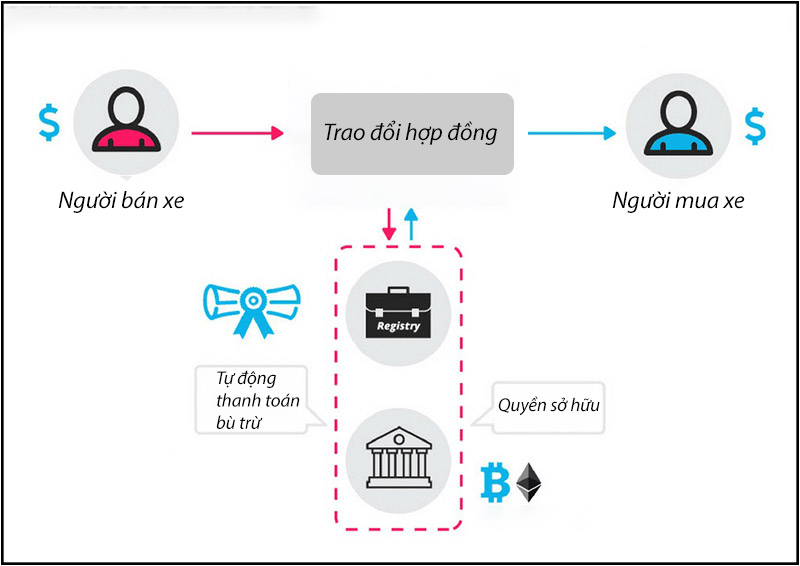
\includegraphics[width=1\textwidth]{Image/smart-contarct.png}
    \caption{Vòng đời của smart-contract}
    \label{fig:smart-contract}
\end{figure}

\newpage
\subsection{Phân tích kiến trúc nền tảng Hyperledger Fabric}

\subsubsection{Mô hình thực thi - sắp xếp - xác thực}
Các mạng blockchain truyền thống như Bitcoin hay Ethereum sử dụng mô hình thực hiện theo thứ tự: trước hết gom và sắp xếp giao dịch, sau đó mới đóng khối và thực thi lại dữ liệu trên từng nút. Mô hình này bộc lộ điểm nghẽn hiệu năng nghiêm ngặt khi tất cả các nút đều phải thực thi lại mọi giao dịch và không đảm bảo tính bảo mật thương mại.
Hyperledger Fabric kiến tạo một kiến trúc đột phá: thực thi trước, sắp xếp sau và xác thực lại \cite{fabric}. Quy trình gồm 3 bước riêng biệt phân rã nhiệm vụ cho từng loại nút chuyên biệt:
\begin{itemize}
    \item \textbf{Thực thi và ký duyệt:} Ứng dụng gửi đề xuất giao dịch đến các nút ký duyệt chỉ định trước. Các nút này chạy thử nghiệm mã hợp đồng thông minh (gọi là chaincode) một cách độc lập trong môi trường bảo mật để tạo ra kết quả đọc/ghi và ký số xác nhận mà không ghi ngay vào sổ cái.
    \item \textbf{Sắp xếp thứ tự:} Ứng dụng thu thập đủ chữ ký phê duyệt từ bước 1 và gửi tập dữ liệu đọc/ghi đến dịch vụ sắp xếp. Các nút sắp xếp chịu trách nhiệm duy nhất là sắp xếp các giao dịch theo đúng trình tự thời gian và đóng gói chúng thành các khối mà không quan tâm bên trong giao dịch chạy logic gì. Điều này tối ưu hóa băng thông mạng cực lớn.
    \item \textbf{Xác thực lại:} Khối được phát tán tới các nút lưu trữ. Các nút này kiểm tra lại xem các chữ ký phê duyệt có hợp lệ và tuân thủ chính sách hay không, đồng thời kiểm tra xem có xung đột dữ liệu đọc/ghi (xung đột song song) hay không. Nếu hợp lệ, giao dịch chính thức được ghi và cập nhật vào cơ sở dữ liệu trạng thái thế giới.
\end{itemize}

\subsubsection{Vấn đề thực tiễn và bài toán tối ưu tài nguyên}
Mặc dù kiến trúc Execute-Order-Validate mang lại hiệu năng cao và phân quyền mạnh mẽ cho doanh nghiệp lớn, tuy nhiên, việc vận hành và triển khai một mạng Hyperledger Fabric chuẩn hóa trong thực tế đối diện với sự phức tạp và cồng kềnh rất lớn về mặt kiến trúc tài nguyên phần cứng hệ thống \cite{fabric}:
\begin{itemize}
    \item \textbf{Hệ thống CA đồ sộ:} Fabric quản lý định danh người dùng và các nút bằng chứng thư số X.509. Mỗi tổ chức tham gia yêu cầu phải duy trì một hoặc nhiều cụm máy chủ CA độc lập, gây quá tải quản trị.
    \item \textbf{Cụm Orderer phức tạp:} Để đảm bảo tính sẵn sàng cao, dịch vụ Orderer phải chạy thuật toán Raft gồm nhiều nút cấu hình phức tạp, đòi hỏi mạng ổn định và độ trễ cực thấp.
    \item \textbf{Cơ sở dữ liệu CouchDB/LevelDB phân tách:} Mỗi nút phải gánh một cơ sở dữ liệu riêng để lưu trữ trạng thái thế giới (thường là CouchDB để hỗ trợ truy vấn JSON nâng cao). Việc đồng bộ hóa dữ liệu liên tục giữa các container CouchDB tiêu tốn lượng RAM và I/O đĩa cứng cực kỳ lớn.
    \item \textbf{Rào cản doanh nghiệp vừa và nhỏ:} Sự phức tạp của việc thiết lập hàng chục container Docker chạy đồng thời (gồm các Peer, Orderer, CA, CouchDB) đòi hỏi hạ tầng máy chủ mạnh mẽ và đội ngũ DevOps trình độ chuyên môn cao. Đối với các doanh nghiệp vừa và nhỏ hoặc các dự án có nguồn lực tài nguyên hạn chế, việc cấu hình và duy trì một hệ thống Fabric đầy đủ cấu hình tiêu chuẩn là một "gánh nặng chi phí" và lãng phí năng lực tính toán.
\end{itemize}

\newpage

\section{Phân tích và Đặc tả yêu cầu hệ thống}
\subsection{Kiến trúc tổng quát}

\subsubsection{Các thay đổi chính}
Để giải quyết bài toán cồng kềnh của các nền tảng blockchain công nghiệp, Khoai Chain được thiết kế theo triết lý tinh gọn, tập trung vào cốt lõi của sổ cái phân tán và loại bỏ các thành phần không cần thiết cho quy mô doanh nghiệp vừa và nhỏ. Các thay đổi mang tính bước ngoặt bao gồm:

\begin{itemize}
    \item \textbf{Tích hợp vai trò nút:} Thay vì phân rã hệ thống thành các nút độc lập (như nút sắp xếp, nút lưu trữ và CA để cấp phép), Khoai Chain tích hợp tất cả các chức năng đồng thuận, định tuyến giao dịch và lưu trữ vào một mô-đun nút duy nhất. Điều này giúp giảm thiểu độ trễ giao tiếp qua mạng lưới và tiết kiệm tối đa RAM/CPU.
    \item \textbf{Cơ chế lưu trữ nhúng:} Thay vì yêu cầu thiết lập các container cơ sở dữ liệu bên ngoài (như CouchDB), sử dụng cơ sở dữ liệu dạng key-value được nhúng trực tiếp vào lõi hệ thống. Quá trình đồng bộ trạng thái sổ cái diễn ra nội bộ, loại bỏ hoàn toàn các cấu hình kết nối mạng phức tạp giữa lõi và cơ sở dữ liệu.
    \item \textbf{Tách biệt hoàn toàn bộ công cụ phát triển hợp đồng thông minh:} Mã nguồn thực thi được tách ra khỏi lõi mạng ngang hàng thông qua bộ công cụ \texttt{khoaichain-sdk}. Sự thay đổi này giúp các nhà phát triển và sinh viên chỉ cần kế thừa các interface có sẵn để viết logic nghiệp vụ, biên dịch và nạp vào mạng lưới mà không cần hiểu sâu về kiến trúc lõi của Khoai Chain.
    \item \textbf{Lược bỏ cơ chế kinh tế:} Do hệ thống phục vụ chuỗi doanh nghiệp nội bộ đã có sự tin tưởng và định danh nhất định, toàn bộ cơ chế khai thác, phí giao dịch và phần thưởng khối đều được loại bỏ để tăng tốc độ đóng gói giao dịch.
\end{itemize}
\newpage
\subsubsection{So sánh với Hyperledger Fabric}
Sự khác biệt cốt lõi giữa Khoai Chain và tiêu chuẩn công nghiệp Hyperledger Fabric được thể hiện chi tiết qua bảng đối chiếu sau:

\begin{table}[H]
    \centering
    \renewcommand{\arraystretch}{1.5}
    \begin{tabular}{|p{3.5cm}|p{5.5cm}|p{5.5cm}|}
        \hline
        \textbf{Tiêu chí} & \textbf{Hyperledger Fabric} & \textbf{Khoai Chain} \\ \hline
        \textbf{Kiến trúc nút} & Phân rã phức tạp (Peer, Orderer, CA hoạt động trên các vùng nhớ riêng). & Tích hợp vai trò nút, với tất cả vai trò xử lý, đồng thuận và lưu trữ nằm trong một tiến trình duy nhất. \\ \hline
        \textbf{Lưu trữ dữ liệu} & Cần hệ quản trị CSDL độc lập (CouchDB/LevelDB chạy khác container). & Tích hợp cơ sở dữ liệu dạng key-value nhúng trực tiếp vào lõi (tiết kiệm I/O). \\ \hline
        \textbf{Phát triển hợp đồng} & Chaincode chạy trong môi trường Docker bị cô lập, cấu hình giao tiếp mạng phức tạp. & Phát triển qua \texttt{khoaichain-sdk} độc lập, dễ dàng biên dịch và thực thi trực tiếp. \\ \hline
        \textbf{Quản lý định danh} & Sử dụng CA với chứng chỉ X.509, yêu cầu duy trì máy chủ CA riêng. & Quản lý tinh gọn qua tệp cấu hình tĩnh (YAML) và cơ chế khóa xác thực nội bộ. \\ \hline
        \textbf{Mức độ triển khai} & Rất nặng. Yêu cầu kiến thức DevOps sâu rộng, tốn nhiều cấu hình YAML/Docker Compose. & Rất nhẹ. Khởi chạy thông qua framework CLI đơn giản hoặc một container duy nhất. \\ \hline
        \textbf{Đối tượng phù hợp} & Tập đoàn lớn, liên minh đa quốc gia, ngân hàng. & Sinh viên nghiên cứu, doanh nghiệp vừa và nhỏ, hệ thống thử nghiệm cục bộ. \\ \hline
    \end{tabular}
    \caption{So sánh đặc tính kỹ thuật giữa Hyperledger Fabric và}
    \label{tab:so_sanh_fabric_khoai}
\end{table}
\newpage
\subsection{Mô hình các chức năng}

Sơ đồ trường hợp sử dụng tổng quát mô tả các tương tác cốt lõi giữa người dùng và hệ thống lõi của mạng lưới. Trong hệ thống này, các tác nhân được chia làm hai nhóm chính: nhóm quản trị hạ tầng (bao gồm quản trị viên mạng, nút cha, nút ngang hàng) và nhóm người dùng cuối (ứng dụng khách).

Cấu trúc phân quyền được thiết kế chặt chẽ nhằm đảm bảo tính phi tập trung nhưng vẫn kiểm soát được vòng đời sinh trưởng của các nút trong mạng. Chi tiết về luồng thực thi và các ràng buộc của từng chức năng được đặc tả cụ thể trong phần dưới đây.

\begin{figure}[H]
    \centering
    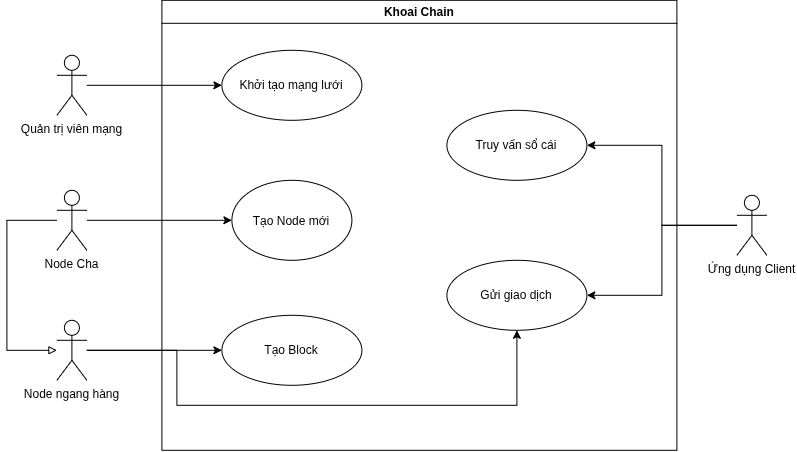
\includegraphics[width=1\textwidth]{USE CASE.drawio.png}
    \caption{Sơ đồ trường hợp sử dụng mạng lưới Khoai Chain}
    \label{fig:usecase_tongquat}
\end{figure}
\newpage
\begin{enumerate}[label=\textbf{\alph*)}]
    \item \textbf{Khởi tạo mạng lưới}
    \begin{table}[H]
        \centering
        \renewcommand{\arraystretch}{1.4}
        \begin{tabularx}{\textwidth}{|p{3.5cm}|X|}
            \hline
            \textbf{Thuộc tính} & \textbf{Mô tả chi tiết} \\ \hline
            \textbf{Tên trường hợp sử dụng} & Khởi tạo mạng lưới \\ \hline
            \textbf{Tác nhân} & Quản trị viên mạng \\ \hline
            \textbf{Tiền điều kiện} & Hệ thống máy chủ được cài đặt mã nguồn lõi. Chưa có dữ liệu sổ cái nào tồn tại. \\ \hline
            \textbf{Luồng sự kiện chính} & 
            1. Quản trị viên cấu hình các tham số mạng cơ bản (thời gian khối, thuật toán đồng thuận) vào tệp cấu hình. \newline
            2. Quản trị viên chạy lệnh khởi tạo trên CLI. \newline
            3. Hệ thống tạo ra khối genesis (khối số 0) chứa định danh của quản trị viên. \newline
            4. Hệ thống ghi khối genesis vào cơ sở dữ liệu cục bộ và mở cổng P2P. \\ \hline
            \textbf{Luồng ngoại lệ} & 
            - Nếu định dạng tệp cấu hình sai: hệ thống báo lỗi và dừng tiến trình. \newline
            - Nếu cổng P2P đã bị chiếm dụng: hệ thống báo lỗi không thể mở kết nối mạng. \\ \hline
            \textbf{Hậu điều kiện} & Mạng lưới được khởi động với 1 nút gốc duy nhất. Sổ cái ở trạng thái sẵn sàng tiếp nhận nút mới. \\ \hline
        \end{tabularx}
        \caption{Đặc tả chi tiết trường hợp sử dụng khởi tạo mạng lưới}
        \label{tab:dac_ta_khoi_tao}
    \end{table}

    \newpage
    
    \item \textbf{Tạo nút mới}
    \begin{table}[H]
        \centering
        \renewcommand{\arraystretch}{1.4} % Giúp các hàng giãn khoảng cách vừa vặn, dễ đọc
        \begin{tabularx}{\textwidth}{|p{3.5cm}|X|}
            \hline
            \textbf{Thuộc tính} & \textbf{Mô tả chi tiết} \\ \hline
            \textbf{Tên trường hợp sử dụng} & Tạo nút mới \\ \hline
            \textbf{Tác nhân} & Quản trị viên mạng, nút cha\\ \hline
            \textbf{Tiền điều kiện} & Mạng lưới đang hoạt động. Tác nhân phải có quyền hợp lệ trên chuỗi để thực hiện cấp phép. \\ \hline
            \textbf{Luồng sự kiện chính} & 
            1. Tác nhân gửi yêu cầu tạo nút con thông qua SDK, kèm theo địa chỉ khóa công khai của nút mới. \newline
            2. Hệ thống kiểm tra chữ ký và cấp bậc của tác nhân trong hợp đồng thông minh. \newline
            3. Hệ thống (bao gồm các nút xác thực) thực hiện đồng thuận để ghi giao dịch cấp phép vào sổ cái. \newline
            4. Nút mới khởi động, kết nối tới nút cha và bắt đầu đồng bộ dữ liệu. \\ \hline
            \textbf{Luồng ngoại lệ} & 
            - Tác nhân không đủ quyền (không phải nút cha): giao dịch bị từ chối, trả về lỗi "Unauthorized". \newline
            - Mạng lưới không đạt đồng thuận: giao dịch cấp phép bị hủy bỏ. \\ \hline
            \textbf{Hậu điều kiện} & Nút mới được định danh hợp lệ trên sổ cái và có thể tham gia vào mạng lưới theo đúng cấp bậc được giao. \\ \hline
        \end{tabularx}
        \caption{Đặc tả chi tiết trường hợp sử dụng tạo nút mới}
        \label{tab:dac_ta_tao_node_moi}
    \end{table}

    \newpage

    \item \textbf{Tạo khối}
    \begin{table}[H]
        \centering
        \renewcommand{\arraystretch}{1.4} % Giúp các hàng giãn khoảng cách vừa vặn, dễ đọc
        \begin{tabularx}{\textwidth}{|p{3.5cm}|X|}
            \hline
            \textbf{Thuộc tính} & \textbf{Mô tả chi tiết} \\ \hline
            \textbf{Tên trường hợp sử dụng} & Tạo khối \\ \hline
            \textbf{Tác nhân} & Nút xác thực \\ \hline
            \textbf{Tiền điều kiện} & Có ít nhất 1 giao dịch hợp lệ đang chờ trong vùng chờ giao dịch. Nút đang ở trạng thái hoạt động. \\ \hline
            \textbf{Luồng sự kiện chính} & 
            1. Nút đến lượt làm trưởng nhóm lấy các giao dịch từ vùng chờ giao dịch. \newline
            2. Nút trưởng nhóm đóng gói giao dịch thành khối đề xuất và phát tán cho các nút xác thực khác. \newline
            3. Các nút xác thực kiểm tra tính hợp lệ của khối và phát tín hiệu bỏ phiếu. \newline
            4. Khi đủ tỷ lệ phiếu đồng ý ($100\%$), khối được chốt. \\ \hline
            \textbf{Luồng ngoại lệ} & 
            - Khối chứa giao dịch sai logic: các nút từ chối bỏ phiếu, khối bị hủy sau thời gian timeout. \newline
            - Nút trưởng nhóm mất kết nối: mạng lưới tự động bầu trưởng nhóm mới. \\ \hline
            \textbf{Hậu điều kiện} & Khối mới được nối vào chuỗi. Trạng thái cơ sở dữ liệu state DB được cập nhật. \\ \hline
        \end{tabularx}
        \caption{Đặc tả chi tiết trường hợp sử dụng tạo khối}
        \label{tab:dac_ta_tao_block}
    \end{table}

    \newpage

    \item \textbf{Gửi giao dịch}
    \begin{table}[H]
        \centering
        \renewcommand{\arraystretch}{1.4} % Giúp các hàng giãn khoảng cách vừa vặn, dễ đọc
        \begin{tabularx}{\textwidth}{|p{3.5cm}|X|}
            \hline
            \textbf{Thuộc tính} & \textbf{Mô tả chi tiết} \\ \hline
            \textbf{Tên trường hợp sử dụng} & Gửi giao dịch \\ \hline
            \textbf{Tác nhân} & Ứng dụng khách \\ \hline
            \textbf{Tiền điều kiện} & Ứng dụng khách có khóa riêng hợp lệ. Kết nối mạng tới ít nhất 1 nút đang mở. \\ \hline
            \textbf{Luồng sự kiện chính} & 
            1. Ứng dụng khách tạo dữ liệu giao dịch nghiệp vụ (ví dụ: tạo lô thuốc) và ký số bằng khóa riêng. \newline
            2. Ứng dụng khách gửi gói tin giao dịch qua API/RPC tới nút tiếp nhận. \newline
            3. Nút tiếp nhận xác thực sơ bộ (chữ ký, định dạng) và đẩy vào vùng chờ giao dịch. \newline
            4. Nút tiếp nhận trả về mã băm cho ứng dụng khách để theo dõi. \\ \hline
            \textbf{Luồng ngoại lệ} & 
            - Chữ ký không hợp lệ: nút tiếp nhận trả về lỗi 400 Bad Request ngay lập tức. \newline
            - Vùng chờ giao dịch đang đầy: nút trả về lỗi 429 Too Many Requests. \\ \hline
            \textbf{Hậu điều kiện} & Giao dịch nằm trong vùng chờ giao dịch, chờ được đóng gói vào khối. \\ \hline
        \end{tabularx}
        \caption{Đặc tả chi tiết trường hợp sử dụng gửi giao dịch}
        \label{tab:dac_ta_gui_giao_dich}
    \end{table}

    \newpage

    \item \textbf{Truy vấn sổ cái}
    \begin{table}[H]
        \centering
        \renewcommand{\arraystretch}{1.4} % Giúp các hàng giãn khoảng cách vừa vặn, dễ đọc
        \begin{tabularx}{\textwidth}{|p{3.5cm}|X|}
            \hline
            \textbf{Thuộc tính} & \textbf{Mô tả chi tiết} \\ \hline
            \textbf{Tên trường hợp sử dụng} & Truy vấn sổ cái \\ \hline
            \textbf{Tác nhân} & Ứng dụng khách \\ \hline
            \textbf{Tiền điều kiện} & Ứng dụng khách kết nối thành công tới nút trong mạng lưới. \\ \hline
            \textbf{Luồng sự kiện chính} & 
            1. Ứng dụng khách gửi yêu cầu đọc dữ liệu (ví dụ: truy xuất thông tin lô thuốc) tới nút. \newline
            2. Nút truy xuất dữ liệu từ state DB cục bộ của mình. \newline
            3. Nút định dạng dữ liệu thành JSON và trả về cho ứng dụng khách. \\ \hline
            \textbf{Luồng ngoại lệ} & 
            - Dữ liệu không tồn tại: nút trả về phản hồi rỗng hoặc thông báo "Not Found". \newline
            - Yêu cầu truy vấn quá lớn (quét toàn bộ chuỗi): nút ngắt kết nối để tránh quá tải. \\ \hline
            \textbf{Hậu điều kiện} & Ứng dụng khách nhận được dữ liệu trạng thái mới nhất từ sổ cái. \\ \hline
        \end{tabularx}
        \caption{Đặc tả chi tiết trường hợp sử dụng truy vấn sổ cái}
        \label{tab:dac_ta_truy_van_so_cai}
    \end{table}
\end{enumerate}

\newpage
\subsection{Các trường hợp sử dụng}
% Cấu trúc danh sách sơ đồ Sequence đã được đồng bộ form
\begin{enumerate}[label=\textbf{\alph*)}]
    \item \textbf{Khởi tạo mạng lưới}
    \begin{figure}[H]
        \centering
        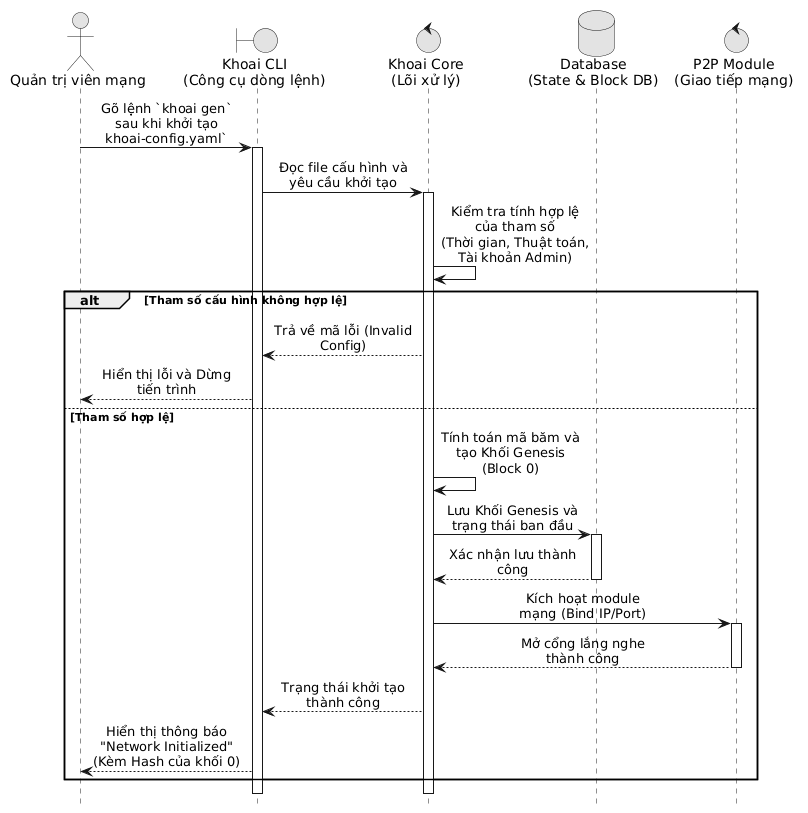
\includegraphics[width=1\textwidth]{Sequence/Khởi tạo.png}
        \caption{Sơ đồ trình tự khởi tạo mạng lưới}
        \label{}
    \end{figure}
    \newpage
    
    \item \textbf{Tạo nút mới}
    \begin{figure}[H]
        \centering
        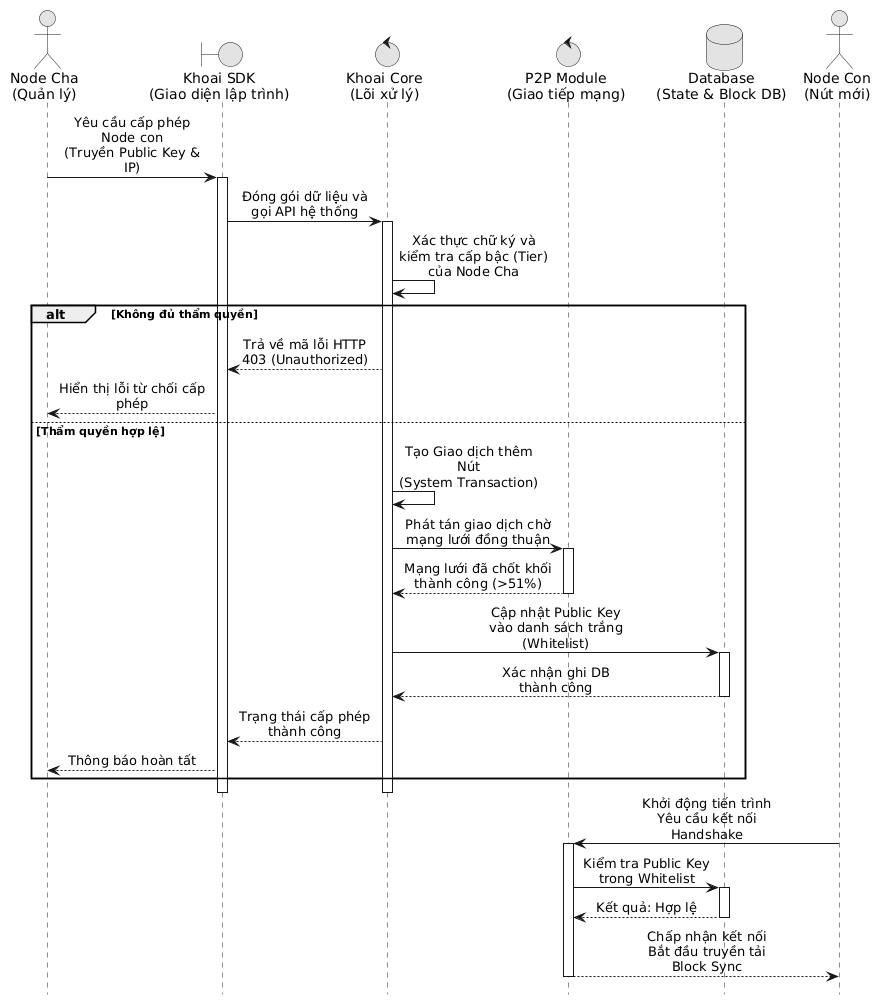
\includegraphics[width=1\textwidth]{Sequence/Tạo node.png}
        \caption{Sơ đồ trình tự tạo nút mới}
        \label{}
    \end{figure}
    \newpage

    \item \textbf{Tạo khối}
    \begin{figure}[H]
        \centering
        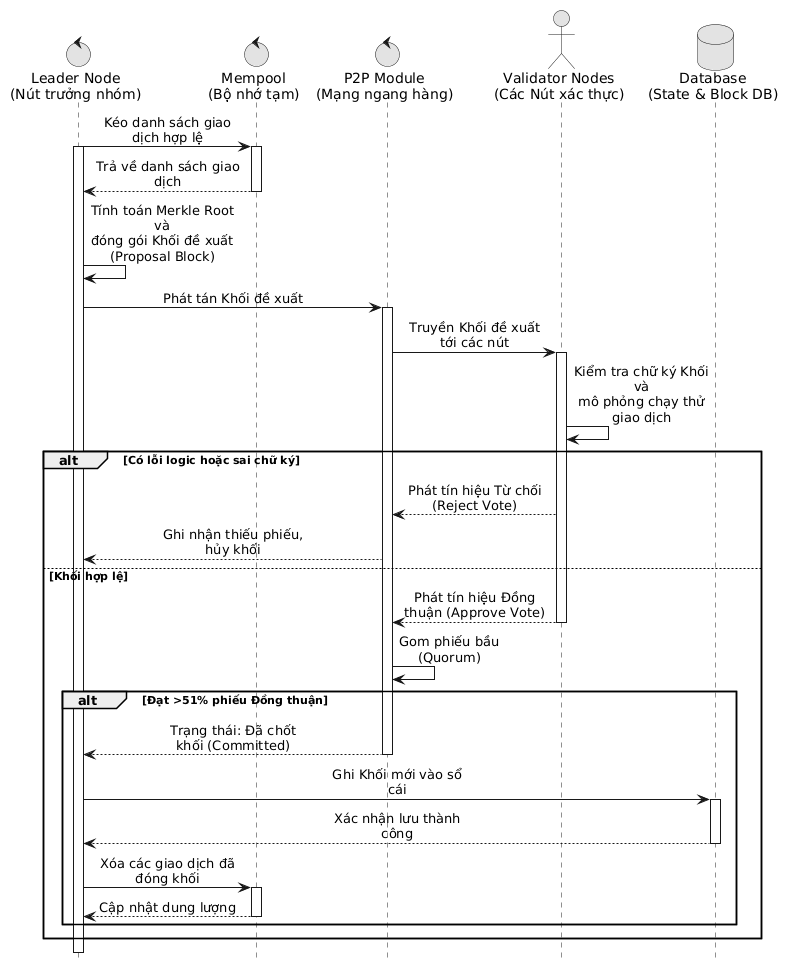
\includegraphics[width=1\textwidth]{Sequence/Tạo block.png}
        \caption{Sơ đồ trình tự tạo khối}
        \label{}
    \end{figure}
    \newpage

    \item \textbf{Gửi giao dịch}
    \begin{figure}[H]
        \centering
        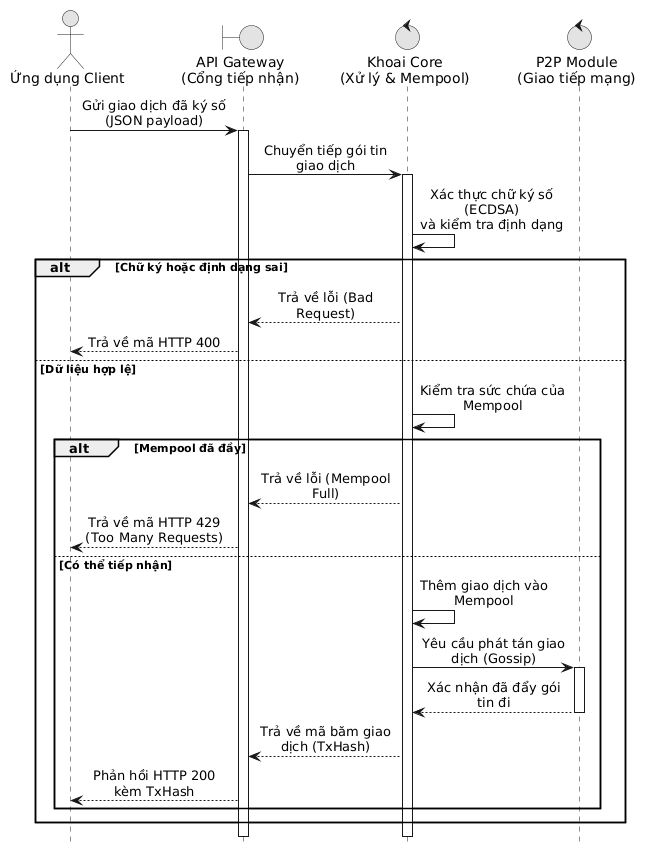
\includegraphics[width=1\textwidth]{Sequence/Tạo giao dịch.png}
        \caption{Sơ đồ trình tự gửi giao dịch}
        \label{}
    \end{figure}
    \newpage

    \item \textbf{Truy vấn sổ cái}
    \begin{figure}[H]
        \centering
        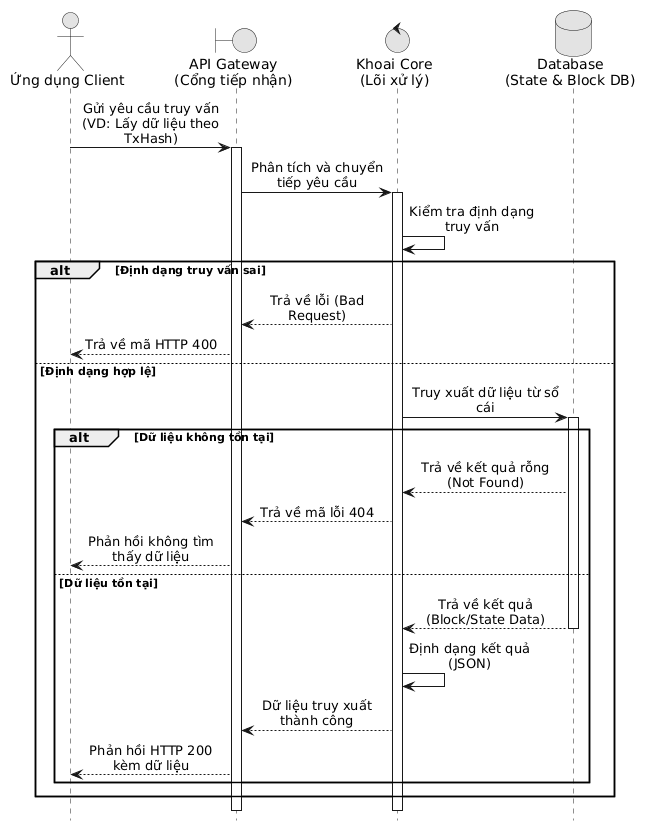
\includegraphics[width=1\textwidth]{Sequence/Truy vấn.png}
        \caption{Sơ đồ trình tự truy vấn sổ cái}
        \label{}
    \end{figure}
\end{enumerate}

\newpage
\subsection{Yêu cầu phi chức năng}

Các yêu cầu phi chức năng đặt ra các tiêu chuẩn về chất lượng, hiệu năng, tính bảo mật và khả năng vận hành của hệ thống, đảm bảo hệ thống đáp ứng tốt các mục tiêu nghiên cứu và thực tiễn đặt ra.

\begin{itemize}
    \item \textbf{Hiệu năng và tốc độ xử lý:} 
    Do hệ thống được thiết kế tinh gọn, loại bỏ các cơ chế đồng thuận nặng nề (như Proof of Work) và sử dụng cơ chế lưu trữ key-value nhúng trực tiếp, thời gian đóng gói và xác thực một khối mới phải đạt tốc độ cao (độ trễ dưới 1 giây khi chạy trên hạ tầng cục bộ). Tốc độ xử lý giao dịch phải đáp ứng mượt mà các bài toán nghiệp vụ nội bộ của doanh nghiệp vừa và nhỏ.

    \item \textbf{Tính bảo mật và toàn vẹn dữ liệu:} 
    Toàn bộ các giao dịch phát sinh từ ứng dụng khách bắt buộc phải được ký số thông qua thuật toán chữ ký số đường cong elliptic (ECDSA/Ed25519). Các nút trong mạng lưới phải thực hiện xác thực chữ ký và kiểm tra tính hợp lệ của gói tin trước khi cho phép đưa vào vùng chờ giao dịch hoặc ghi vào sổ cái. Dữ liệu trên chuỗi phải đảm bảo tính bất biến, không thể giả mạo hay chỉnh sửa nhờ cơ chế liên kết mã băm.

    \item \textbf{Khả năng mở rộng và tính sẵn sàng của mạng ngang hàng:} 
    Mạng lưới ngang hàng phải hỗ trợ cơ chế tự động khám phá và kết nối giữa các nút thông qua giao thức truyền bá thông điệp. Khi có một nút mới gia nhập hoặc ngắt kết nối đột ngột, các nút còn lại phải tự động cập nhật cấu trúc mạng và đồng bộ trạng thái sổ cái một cách nhanh chóng mà không làm gián đoạn toàn bộ hệ thống.

    \item \textbf{Tính tối ưu tài nguyên:} 
    Khác với các nền tảng blockchain công nghiệp đòi hỏi cấu hình phần cứng lớn, phải tối ưu hóa mức tiêu thụ tài nguyên (CPU, RAM và dung lượng ổ cứng). Một nút hệ thống phải có khả năng khởi chạy ổn định ngay cả trên các thiết bị máy tính cá nhân hoặc máy chủ ảo cấu hình thấp, phục vụ hiệu quả cho môi trường thử nghiệm và giáo dục.

    \item \textbf{Tính độc lập và dễ triển khai:} 
    Kiến trúc mã nguồn phải được tách biệt rõ ràng giữa tầng lõi và bộ công cụ phát triển. Quá trình triển khai mạng lưới phải được tự động hóa thông qua công nghệ container hóa, cho phép người dùng khởi chạy và cấu hình toàn bộ hệ thống chỉ thông qua một vài thao tác lệnh cơ bản.
\end{itemize}\newpage

\section{Thiết kế kiến trúc}

\subsection{Kiến trúc tổng thể hệ thống}
Hệ thống Khoai Chain được thiết kế theo mô hình kiến trúc tích hợp nhằm tối ưu hóa tài nguyên phần cứng và giảm thiểu độ trễ mạng trong môi trường doanh nghiệp. Mỗi một nút trong mạng lưới là một thực thể độc lập chứa đầy đủ ba phân hệ cốt lõi: mô-đun mạng ngang hàng, lõi blockchain và hệ thống quản lý hợp đồng thông minh.

Khác với kiến trúc phân rã của Hyperledger Fabric, Khoai Chain đóng gói toàn bộ quy trình từ tiếp nhận giao dịch, đóng khối cho đến cập nhật trạng thái cơ sở dữ liệu vào một tiến trình duy nhất. Hệ thống sử dụng cơ sở dữ liệu dạng key-value (như LevelDB/BadgerDB) được nhúng trực tiếp, giúp loại bỏ hoàn toàn chi phí I/O khi phải giao tiếp với các container cơ sở dữ liệu bên ngoài. Toàn bộ kiến trúc được module hóa rõ ràng, cho phép dễ dàng mở rộng và bảo trì.

\subsection{Thiết kế mô-đun P2P}
Mô-đun P2P chịu trách nhiệm duy trì kết nối mạng lưới và đồng bộ hóa trạng thái toàn cục giữa các nút. Kiến trúc P2P được chia thành 4 thành phần chính:
\begin{itemize}
    \item \textbf{Máy chủ và nút:} Thành phần \texttt{Server} quản lý vòng đời của các kết nối TCP/IP hoặc WebSocket, liên tục lắng nghe các yêu cầu từ mạng. Mỗi kết nối với một nút khác được trừu tượng hóa thành một đối tượng \texttt{Peer}, lưu trữ định danh (khóa công khai) và trạng thái đồng bộ hiện tại.
    \item \textbf{Thông điệp:} Dữ liệu truyền tải giữa các nút được chuẩn hóa dưới định dạng JSON. Bản tin cơ sở bao gồm trường \texttt{Type} (như \texttt{MsgNewBlock}, \texttt{MsgSendChain}) và phần \texttt{Payload}. Thiết kế này giúp hệ thống dễ dàng phân loại và định tuyến gói tin.
    \item \textbf{Bộ xử lý:} Đóng vai trò là bộ định tuyến logic. Khi nhận được bản tin, bộ xử lý sẽ kiểm tra tính hợp lệ của dữ liệu và kích hoạt các quy trình tương ứng. Đặc biệt, trong quá trình đồng bộ chuỗi (\texttt{MsgSendChain}), bộ xử lý áp dụng cơ chế xác thực lô. Nó sẽ rà soát tính liên tục của mảng các khối nhận được (đảm bảo \texttt{PrevBlockHash} khớp hoàn toàn) trước khi cho phép ghi đè xuống cơ sở dữ liệu, ngăn chặn tuyệt đối tình trạng rác hóa cơ sở dữ liệu.
\end{itemize}
\newpage
\subsection{Thiết kế lõi blockchain}
\subsubsection{Cấu trúc dữ liệu khối và giao dịch}
Cấu trúc dữ liệu của Khoai Chain được thiết kế tối giản nhưng vẫn tuân thủ nghiêm ngặt các tiêu chuẩn mật mã học:
\begin{itemize}
    \item \textbf{Giao dịch:} Là đơn vị thay đổi trạng thái cơ bản. Mỗi giao dịch chứa: \texttt{ID} (mã băm giao dịch), \texttt{Timestamp}, và \textbf{Payload}. Trong payload chứa thông tin định danh người gửi (\texttt{Sender}), tên hợp đồng (\texttt{Contract}), hàm gọi (\texttt{Function}), tham số (\texttt{Args}), giá trị \texttt{Nonce} chống tấn công phát lại và chữ ký số (\texttt{Signature}) sử dụng thuật toán Ed25519.
    \item \textbf{Khối:} Đóng gói các giao dịch hợp lệ. Khối bao gồm \texttt{Height} (độ cao chuỗi), \texttt{Timestamp}, danh sách các giao dịch và \texttt{PrevBlockHash} (mã băm của khối liền trước). Mã băm của khối hiện tại (\texttt{Hash}) được tính toán bằng thuật toán SHA-256 dựa trên việc tuần tự hóa toàn bộ dữ liệu khối, sau đó lưu trữ dưới dạng chuỗi hệ thập lục phân. Điểm đặc biệt của kiến trúc là khối khởi thủy được cấu hình mang tính tất định tuyệt đối, đảm bảo mọi nút khởi chạy đều chung một điểm gốc toán học.
\end{itemize}

\subsubsection{Luồng hoạt động của vùng chờ giao dịch}
Vùng chờ giao dịch là nơi lưu trữ tạm thời các giao dịch chưa được xác nhận. Luồng xử lý của vùng chờ này được thiết kế cực kỳ chặt chẽ:
\begin{enumerate}
    \item \textbf{Tiếp nhận và xác thực sơ bộ:} Khi một giao dịch mới được gửi đến, vùng chờ kiểm tra định dạng chữ ký số Ed25519 bằng khóa công khai của người gửi. Nếu chữ ký sai lệch, giao dịch bị loại bỏ ngay tại viền mạng.
    \item \textbf{Trạng thái chờ:} Các giao dịch hợp lệ được đẩy vào hàng đợi trong RAM để chuẩn bị đóng gói.
    \item \textbf{Dọn dẹp tự động:} Ngay khi một khối mới được đóng thành công hoặc được đồng bộ từ mạng ngang hàng (\texttt{AddBlocks}), hệ thống sẽ quét qua danh sách các giao dịch nằm trong khối đó và gọi hàm \texttt{RemoveIncluded} để xóa chúng khỏi vùng chờ, giải phóng bộ nhớ và tránh việc thực thi trùng lặp.
\end{enumerate}

\subsection{Thiết kế hệ thống hợp đồng thông minh}
Hệ thống hợp đồng thông minh của Khoai Chain được thiết kế để tách biệt hoàn toàn trạng thái tính toán và trạng thái lưu trữ vĩnh viễn:
\begin{itemize}
    \item \textbf{Trình quản lý hợp đồng:} Là trái tim của hệ thống thực thi, quản lý trạng thái máy tự động. Trình quản lý cung cấp hai cơ chế cốt lõi: \texttt{ExecuteOnly} và \texttt{Commit}. 
    \item \textbf{Luồng thực thi an toàn:} Khi xác thực một lô giao dịch từ mạng gửi về, hệ thống sử dụng \texttt{ExecuteOnly} để tính toán các logic nghiệp vụ. Kết quả thay đổi (state changes) chỉ được lưu tạm vào vùng nhớ đệm (\texttt{stagingState}). Nhờ vậy, nếu có bất kỳ giao dịch nào trong lô gây ra lỗi (như vi phạm quyền truy cập, sai logic hợp đồng), toàn bộ tiến trình có thể bị hủy bỏ mà không làm "bẩn" cơ sở dữ liệu chính.
    \item \textbf{Chốt trạng thái:} Chỉ khi toàn bộ các bước kiểm tra mật mã học và logic hợp đồng hoàn tất không có lỗi, hàm \texttt{Commit} mới được gọi. Lúc này, \texttt{stagingState} mới chính thức được ghi đè xuống cơ sở dữ liệu, đảm bảo tính nguyên tử của hệ thống.
    \item \textbf{Bộ định tuyến:} Đóng vai trò ánh xạ tên hợp đồng và tên hàm từ giao dịch tới các đoạn mã Go đã được biên dịch tương ứng trong hệ thống.
\end{itemize}

\subsection{Cơ chế đồng thuận}
Do đặc thù hướng tới chuỗi doanh nghiệp nội bộ với các định danh có độ tin cậy nhất định, Khoai Chain không sử dụng mô hình bằng chứng công việc (PoW) nhằm tiết kiệm năng lượng. Thay vào đó, hệ thống tập trung vào tính toàn vẹn của chuỗi và luật chuỗi dài nhất kết hợp với ràng buộc phả hệ tuyến tính:
\begin{itemize}
    \item \textbf{Đồng thuận dữ liệu gốc:} Các nút phải đạt được sự thống nhất tuyệt đối về khối khởi thủy. Bất kỳ sự khác biệt nào ở điểm khởi đầu đều khiến chuỗi bị mạng lưới từ chối.
    \item \textbf{Luật gắn kết khối:} Cơ chế đồng thuận cốt lõi nằm ở bước kiểm duyệt khối. Khi một nút đề xuất một lô khối mới, các nút xác thực không chỉ kiểm tra độ cao (\texttt{Height}), mà bắt buộc phải dò ngược mã băm (\texttt{PrevBlockHash}) để đảm bảo khối mới thực sự kế thừa từ chính khối đỉnh hiện tại (\texttt{LastHash}) lưu trong cơ sở dữ liệu.
    \item \textbf{Chống phân nhánh đa đầu:} Nếu phát hiện khối mới không gắn với tổ tiên cục bộ, hoặc lô khối chứa mắt xích đứt gãy, hệ thống sẽ tự động vô hiệu hóa toàn bộ quá trình đồng bộ lô (\texttt{Atomic Batch Rejection}). Điều này giải quyết triệt để nguy cơ hệ thống bị rẽ nhánh song song, đảm bảo sổ cái luôn duy trì ở trạng thái là một chuỗi đơn nhất và minh bạch.
\end{itemize}
\newpage

\section{Hướng dẫn sử dụng và Triển khai}

\subsection{Khởi tạo môi trường và cấu hình}
Để hệ thống vận hành trơn tru, người dùng cần chuẩn bị một môi trường tối giản bao gồm Docker Engine và Go runtime \cite{donovan}. Toàn bộ thiết lập mạng lưới được tập trung vào một tệp cấu hình duy nhất nhằm giảm tải công việc của quản trị viên.

\begin{itemize}
    \item \textbf{Cấu hình mạng lưới qua \texttt{khoai-config.yaml}:} Tệp cấu hình này định nghĩa toàn bộ cấu trúc mạng, bao gồm thông tin định danh của các nút (mã định danh nút), địa chỉ IP, cổng giao tiếp P2P và các tham số cốt lõi của chuỗi (như thời gian đóng khối tối đa, kích thước khối). Việc sử dụng định dạng YAML giúp các cấu hình trở nên trực quan và dễ dàng chỉnh sửa cho người dùng mới.
    \item \textbf{Quản lý phiên bản:} Để tránh rủi ro phân nhánh mạng do lệch logic xử lý khối, hệ thống kiểm soát phiên bản lõi chặt chẽ. Mỗi gói tin gửi đi qua mạng ngang hàng đều đính kèm cờ phiên bản. Nếu phát hiện sự không tương thích (ví dụ: một nút chạy lõi v1.0 cố gắng kết nối với mạng v2.0), kết nối P2P sẽ bị từ chối ngay từ vòng bắt tay.
\end{itemize}

\subsection{Chạy thử nghiệm bằng CLI và Docker}
Một trong những điểm mạnh cốt lõi của Khoai Chain là trải nghiệm dành cho nhà phát triển (DX) thông qua sự kết hợp giữa kiến trúc container và công cụ dòng lệnh (CLI).

\begin{itemize}
    \item \textbf{Khởi chạy hạ tầng qua Docker:} Thay vì cài đặt từng thành phần cơ sở dữ liệu và biến môi trường phức tạp, người dùng chỉ cần một lệnh \texttt{docker-compose up -d}. Lệnh này sẽ tự động khởi tạo các container chứa lõi blockchain, gắn các vùng nhớ dữ liệu cục bộ và thiết lập mạng nội bộ ảo cho các nút giao tiếp với nhau.
    \item \textbf{Tương tác qua SDK Khoai Chain:} Để tương tác với mạng lưới, người dùng không cần phải chui trực tiếp vào từng container. Bộ SDK được thiết kế dưới dạng công cụ CLI tiện lợi, cho phép thực thi các lệnh gọi nhanh (như truy vấn số dư, gửi giao dịch). Bản chất các lệnh CLI này hoạt động như một cầu nối ứng dụng khách gọn nhẹ, kết nối và thực thi lệnh trực tiếp trên hạ tầng Docker đang vận hành ngầm, mang lại cảm giác mượt mà và trực quan.
\end{itemize}

\subsection{Kịch bản chạy thử nghiệm mẫu cho sinh viên}
Nhằm phục vụ mục đích giáo dục, Khoai Chain cung cấp một kịch bản "Hello World" hoàn chỉnh, giúp sinh viên làm quen với kiến trúc blockchain chỉ trong vòng 15 phút:
\begin{enumerate}
    \item \textbf{Bước 1 - Khởi động mạng:} Sinh viên sử dụng tệp \texttt{docker-compose.yaml} mẫu để dựng một mạng riêng nhỏ gồm 3 nút ngang hàng.
    \item \textbf{Bước 2 - Khởi tạo hợp đồng thông minh:} Sử dụng mã nguồn Go mẫu do hệ thống cung cấp (ví dụ: hợp đồng quản lý chứng chỉ học tập), sinh viên sẽ đọc hiểu cấu trúc interface của hợp đồng.
    \item \textbf{Bước 3 - Triển khai và gửi giao dịch:} Sử dụng công cụ CLI để gửi một giao dịch cấp phát chứng chỉ lên mạng. Màn hình console sẽ hiển thị luồng log trực tiếp: giao dịch được đưa vào vùng chờ giao dịch $\rightarrow$ đóng khối $\rightarrow$ đồng bộ P2P.
    \item \textbf{Bước 4 - Truy vấn kết quả:} Sinh viên sử dụng CLI kết nối ngẫu nhiên vào một nút khác trong mạng để truy vấn thông tin chứng chỉ vừa tạo, qua đó trực tiếp kiểm chứng đặc tính đồng bộ và phân tán của sổ cái.
\end{enumerate}

\subsection{Các chức năng đang phát triển và Hạn chế hiện tại}
Dù đã đáp ứng được mô hình blockchain riêng biệt tinh gọn, ở phiên bản hiện tại vẫn tồn tại một số giới hạn kỹ thuật cần được khắc phục trong các giai đoạn nghiên cứu tiếp theo:
\begin{itemize}
    \item \textbf{Khả năng tự động khám phá nút:} Mạng lưới hiện tại đang dựa vào cơ chế định tuyến tĩnh thông qua IP được cấu hình sẵn trong Docker. Trong tương lai, hệ thống cần tích hợp giao thức DHT để các nút có thể tự động tìm thấy nhau trên môi trường Internet mở.
    \item \textbf{Cơ chế hoàn tác và tái sắp xếp chuỗi phức tạp:} Hệ thống hiện tại đã ngăn chặn được các nhánh rác khi đồng bộ, nhưng nếu mạng bị đứt gãy vật lý và tạo ra hai chuỗi song song dài bằng nhau, chưa có cơ chế hồi phục toàn diện để tự động gỡ bỏ các khối bị sai lệch và đưa toàn mạng về một trạng thái đồng thuận duy nhất.
    \item \textbf{Bảo mật tính toán trong hợp đồng thông minh:} Môi trường thực thi hợp đồng thông minh hiện chưa được cô lập tài nguyên tuyệt đối. Một hợp đồng chứa vòng lặp vô hạn do lập trình viên sơ suất có thể làm cạn kiệt tài nguyên CPU của tiến trình lõi. Cơ chế giới hạn tính toán đang được nghiên cứu và phát triển.
\end{itemize}
\newpage

% Phần kết luận không đánh số chương
\section*{Kết luận}
\addcontentsline{toc}{section}{Kết luận}

\subsection*{Tóm tắt các chức năng }
\addcontentsline{toc}{subsection}{Tóm tắt các chức năng}
Đồ án đã hoàn thành mục tiêu nghiên cứu và xây dựng thành công – một nền tảng blockchain riêng tư tinh gọn, giải quyết triệt để sự cồng kềnh của các hệ thống công nghiệp như Hyperledger Fabric. Tính đến giai đoạn hiện tại, hệ thống đã hoàn thiện và chốt hạ các chức năng cốt lõi sau:

\begin{itemize}
    \item \textbf{Lõi blockchain và cơ sở dữ liệu nhúng:} Tự xây dựng toàn bộ cấu trúc dữ liệu khối và giao dịch từ con số không bằng ngôn ngữ Go \cite{donovan}. Tích hợp thành công cơ sở dữ liệu key-value nhúng để lưu trữ trạng thái sổ cái, đảm bảo tốc độ truy xuất I/O tối ưu mà không cần phụ thuộc vào hệ quản trị cơ sở dữ liệu bên ngoài.
    \item \textbf{Mạng ngang hàng đồng bộ:} Triển khai thành công giao thức truyền tải bản tin và xử lý đồng bộ chuỗi. Đã giải quyết triệt để rủi ro phân nhánh đa đầu bằng cơ chế kiểm duyệt phả hệ tuyến tính nghiêm ngặt và đồng nhất hóa khối khởi thủy.
    \item \textbf{Quản lý vùng chờ giao dịch và hợp đồng thông minh:} Hoàn thiện luồng thực thi giao dịch an toàn với cơ chế tách biệt vùng nhớ đệm. Hệ thống chỉ chốt trạng thái sổ cái khi toàn bộ lô khối hợp lệ, loại bỏ rủi ro dữ liệu rác.
    \item \textbf{Triển khai container hóa và SDK:} Đóng gói thành công tiến trình nút vào môi trường Docker và xây dựng bộ công cụ giao diện dòng lệnh, cho phép khởi chạy, quản trị và tương tác với mạng lưới chỉ qua các thao tác lệnh đơn giản.
\end{itemize}

\subsection*{Định hướng hoàn thiện mã nguồn}
\addcontentsline{toc}{subsection}{Định hướng hoàn thiện mã nguồn}
Dựa trên nền tảng kiến trúc đã thiết lập, để thực sự sẵn sàng cho môi trường triển khai thực tế của doanh nghiệp, mã nguồn cần tiếp tục được nghiên cứu và nâng cấp ở các khía cạnh sau:

\begin{itemize}
    \item \textbf{Hoàn thiện cơ chế tái sắp xếp chuỗi:} Bổ sung thuật toán hoàn tác tự động. Trong trường hợp mạng lưới gặp sự cố chia cắt sinh ra các nhánh tạm thời, hệ thống phải có khả năng tự động so sánh, loại bỏ các khối thuộc nhánh ngắn hơn và đồng bộ lại theo nhánh chính thức khi mạng kết nối lại.
    \item \textbf{Bảo vệ môi trường thực thi hợp đồng:} Cài đặt cơ chế giới hạn tài nguyên (như áp dụng \texttt{context.WithTimeout} trong Go) để tự động ngắt các hợp đồng thông minh bị lỗi vòng lặp vô hạn, ngăn chặn tình trạng cạn kiệt tài nguyên CPU của nút tiếp nhận.
    \item \textbf{Tối ưu hóa khả năng lưu trữ:} Khi hệ thống vận hành lâu dài, kích thước sổ cái sẽ phình to. Cần nghiên cứu phát triển cơ chế nén hoặc dọn dẹp dữ liệu lịch sử nhưng vẫn giữ lại các bằng chứng mật mã để đảm bảo các nút có cấu hình thấp vẫn có thể tham gia lưu trữ mà không bị tràn bộ nhớ đệm.
    \item \textbf{Cơ chế bảo mật dữ liệu riêng tư:} Nâng cấp kiến trúc luồng dữ liệu để hỗ trợ các giao dịch ẩn danh giữa một nhóm nút cụ thể trong mạng. Điều này giúp các doanh nghiệp trong cùng chuỗi có thể giao dịch nội bộ mà không làm lộ chi tiết hợp đồng ra toàn bộ phần còn lại của mạng lưới.
    \item \textbf{Phát triển giao diện API kiểm thử nhanh:} Tích hợp một module máy chủ web hạng nhẹ mở cổng giao tiếp HTTP/RESTful trực tiếp vào nút. Phân hệ này sẽ cung cấp một giao diện trực quan giúp các nhà phát triển dễ dàng gửi giao dịch, gọi thử các hàm hợp đồng thông minh và xem log trạng thái thay đổi theo thời gian thực mà không cần phụ thuộc hoàn toàn vào giao diện dòng lệnh.
\end{itemize}

\newpage


\addcontentsline{toc}{section}{Tài liệu tham khảo}
\renewcommand{\refname}{Tài liệu tham khảo}
\begin{thebibliography}{99}

% Tai lieu cho phan ly thuyet Blockchain va P2P
\bibitem{antonopoulos}
A. M. Antonopoulos, \textit{Mastering Bitcoin: Programming the Open Blockchain}, 2nd ed. Sebastopol, CA: O'Reilly Media, 2017.

\bibitem{fabric}
E. Androulaki et al., "Hyperledger fabric: a distributed operating system for permissioned blockchains," in \textit{Proceedings of the Thirteenth EuroSys Conference}, Porto, Portugal, 2018, pp. 1-15.

\bibitem{lamport}
L. Lamport, R. Shostak, and M. Pease, "The Byzantine Generals Problem," \textit{ACM Transactions on Programming Languages and Systems}, vol. 4, no. 3, pp. 382-401, 1982.

\bibitem{castro}
M. Castro and B. Liskov, "Practical Byzantine Fault Tolerance," in \textit{Proceedings of the Third Symposium on Operating Systems Design and Implementation}, New Orleans, LA, 1999, pp. 173-186.

\bibitem{ongaro}
D. Ongaro and J. Ousterhout, "In search of an understandable consensus algorithm," in \textit{2014 USENIX Annual Technical Conference}, Philadelphia, PA, 2014, pp. 305-319.

\bibitem{demers}
A. Demers et al., "Epidemic algorithms for replicated database maintenance," in \textit{Proceedings of the sixth annual ACM Symposium on Principles of distributed computing}, Vancouver, BC, Canada, 1987, pp. 1-12.

\bibitem{stallings}
W. Stallings, \textit{Cryptography and Network Security: Principles and Practice}, 7th ed. London, UK: Pearson, 2017.

\bibitem{bernstein}
D. J. Bernstein et al., "High-speed high-security signatures," \textit{Journal of Cryptographic Engineering}, vol. 2, no. 2, pp. 77-89, 2012.

\bibitem{donovan}
A. A. A. Donovan and B. W. Kernighan, \textit{The Go Programming Language}. Boston, MA: Addison-Wesley Professional, 2015.

\end{thebibliography}

\end{document}
